\chapter{Simulation}
Die Simulationen sind vom Grundaufbau her wie folgt implementiert: Sie bestehen aus einem Konfigurationsskript, das die Parameter für das eigentliche Modell in den Matlab Workspace lädt und die Automatisierung der Simulationsläufe implementiert. Das Modell wird in Simulink über das PLECS Blockset aufgebaut und die Daten werden über eine Ausgabe als gebündelte Schnittstelle an Matlab zurückgegeben. Die Rückführung der Daten erfolgt einheitlich für die Simulationen in einer festgelegten Reihenfolge, siehe Abb. \ref{fig:plecsout}. Dies ermöglicht eine einheitliche Auswertung und Speicherung der Daten, zur Begrenzung der Datenmenge wird die Anzahl der Messpunkte auf die letzte Sinusperiode begrenzt. Die Schaltung und die zugehörige Steuerung befinden sich in jeweils eigenen PLECS-Systemen, für das Netz und den Elektrolyseur ist ein eigenes Subsystem vorgesehen, siehe Abbildung \ref{fig:plecssimulationsaufbau}.
\begin{figure} [H]
\centering
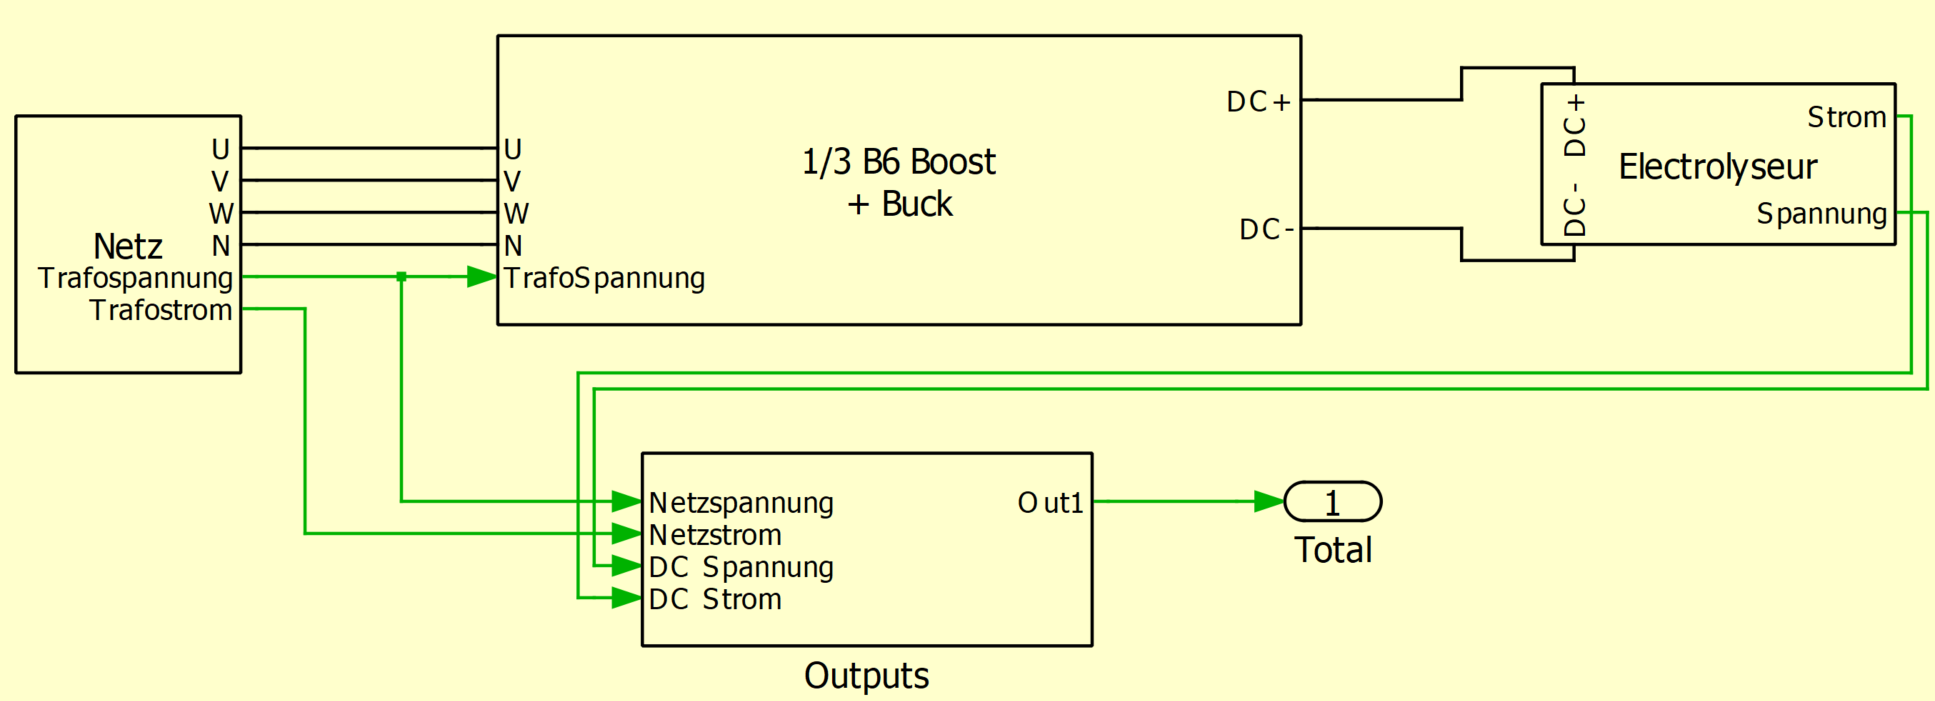
\includegraphics[width=1\linewidth]{content/Grafiken/PLECS_Simulationsaufbau}
\caption{Übersicht der PLECS Simulation}
\label{fig:plecssimulationsaufbau}
\end{figure}
Das Netz wird durch eine einfache Drehstromquelle dargestellt und kann in späteren Schritten durch Netzimpedanzen und Fehlerszenarien ergänzt werden. Der Elektrolyseur besteht der Einfachheit halber aus einem geeigneten Lastwiderstand, der im Betriebspunkt die gemäß Skript eingestellte Leistung aufnimmt. Zusätzlich werden Widerstände eingesetzt, um die Schaltung in \gls{PLECS} berechenbar zu machen, da sonst beim Einschaltvorgang durch Kapazitäten unendlich hohe Ströme entstehen würden. In der realen Anwendung treten diese als parasitäre Widerstände auf.
\begin{figure}
\centering
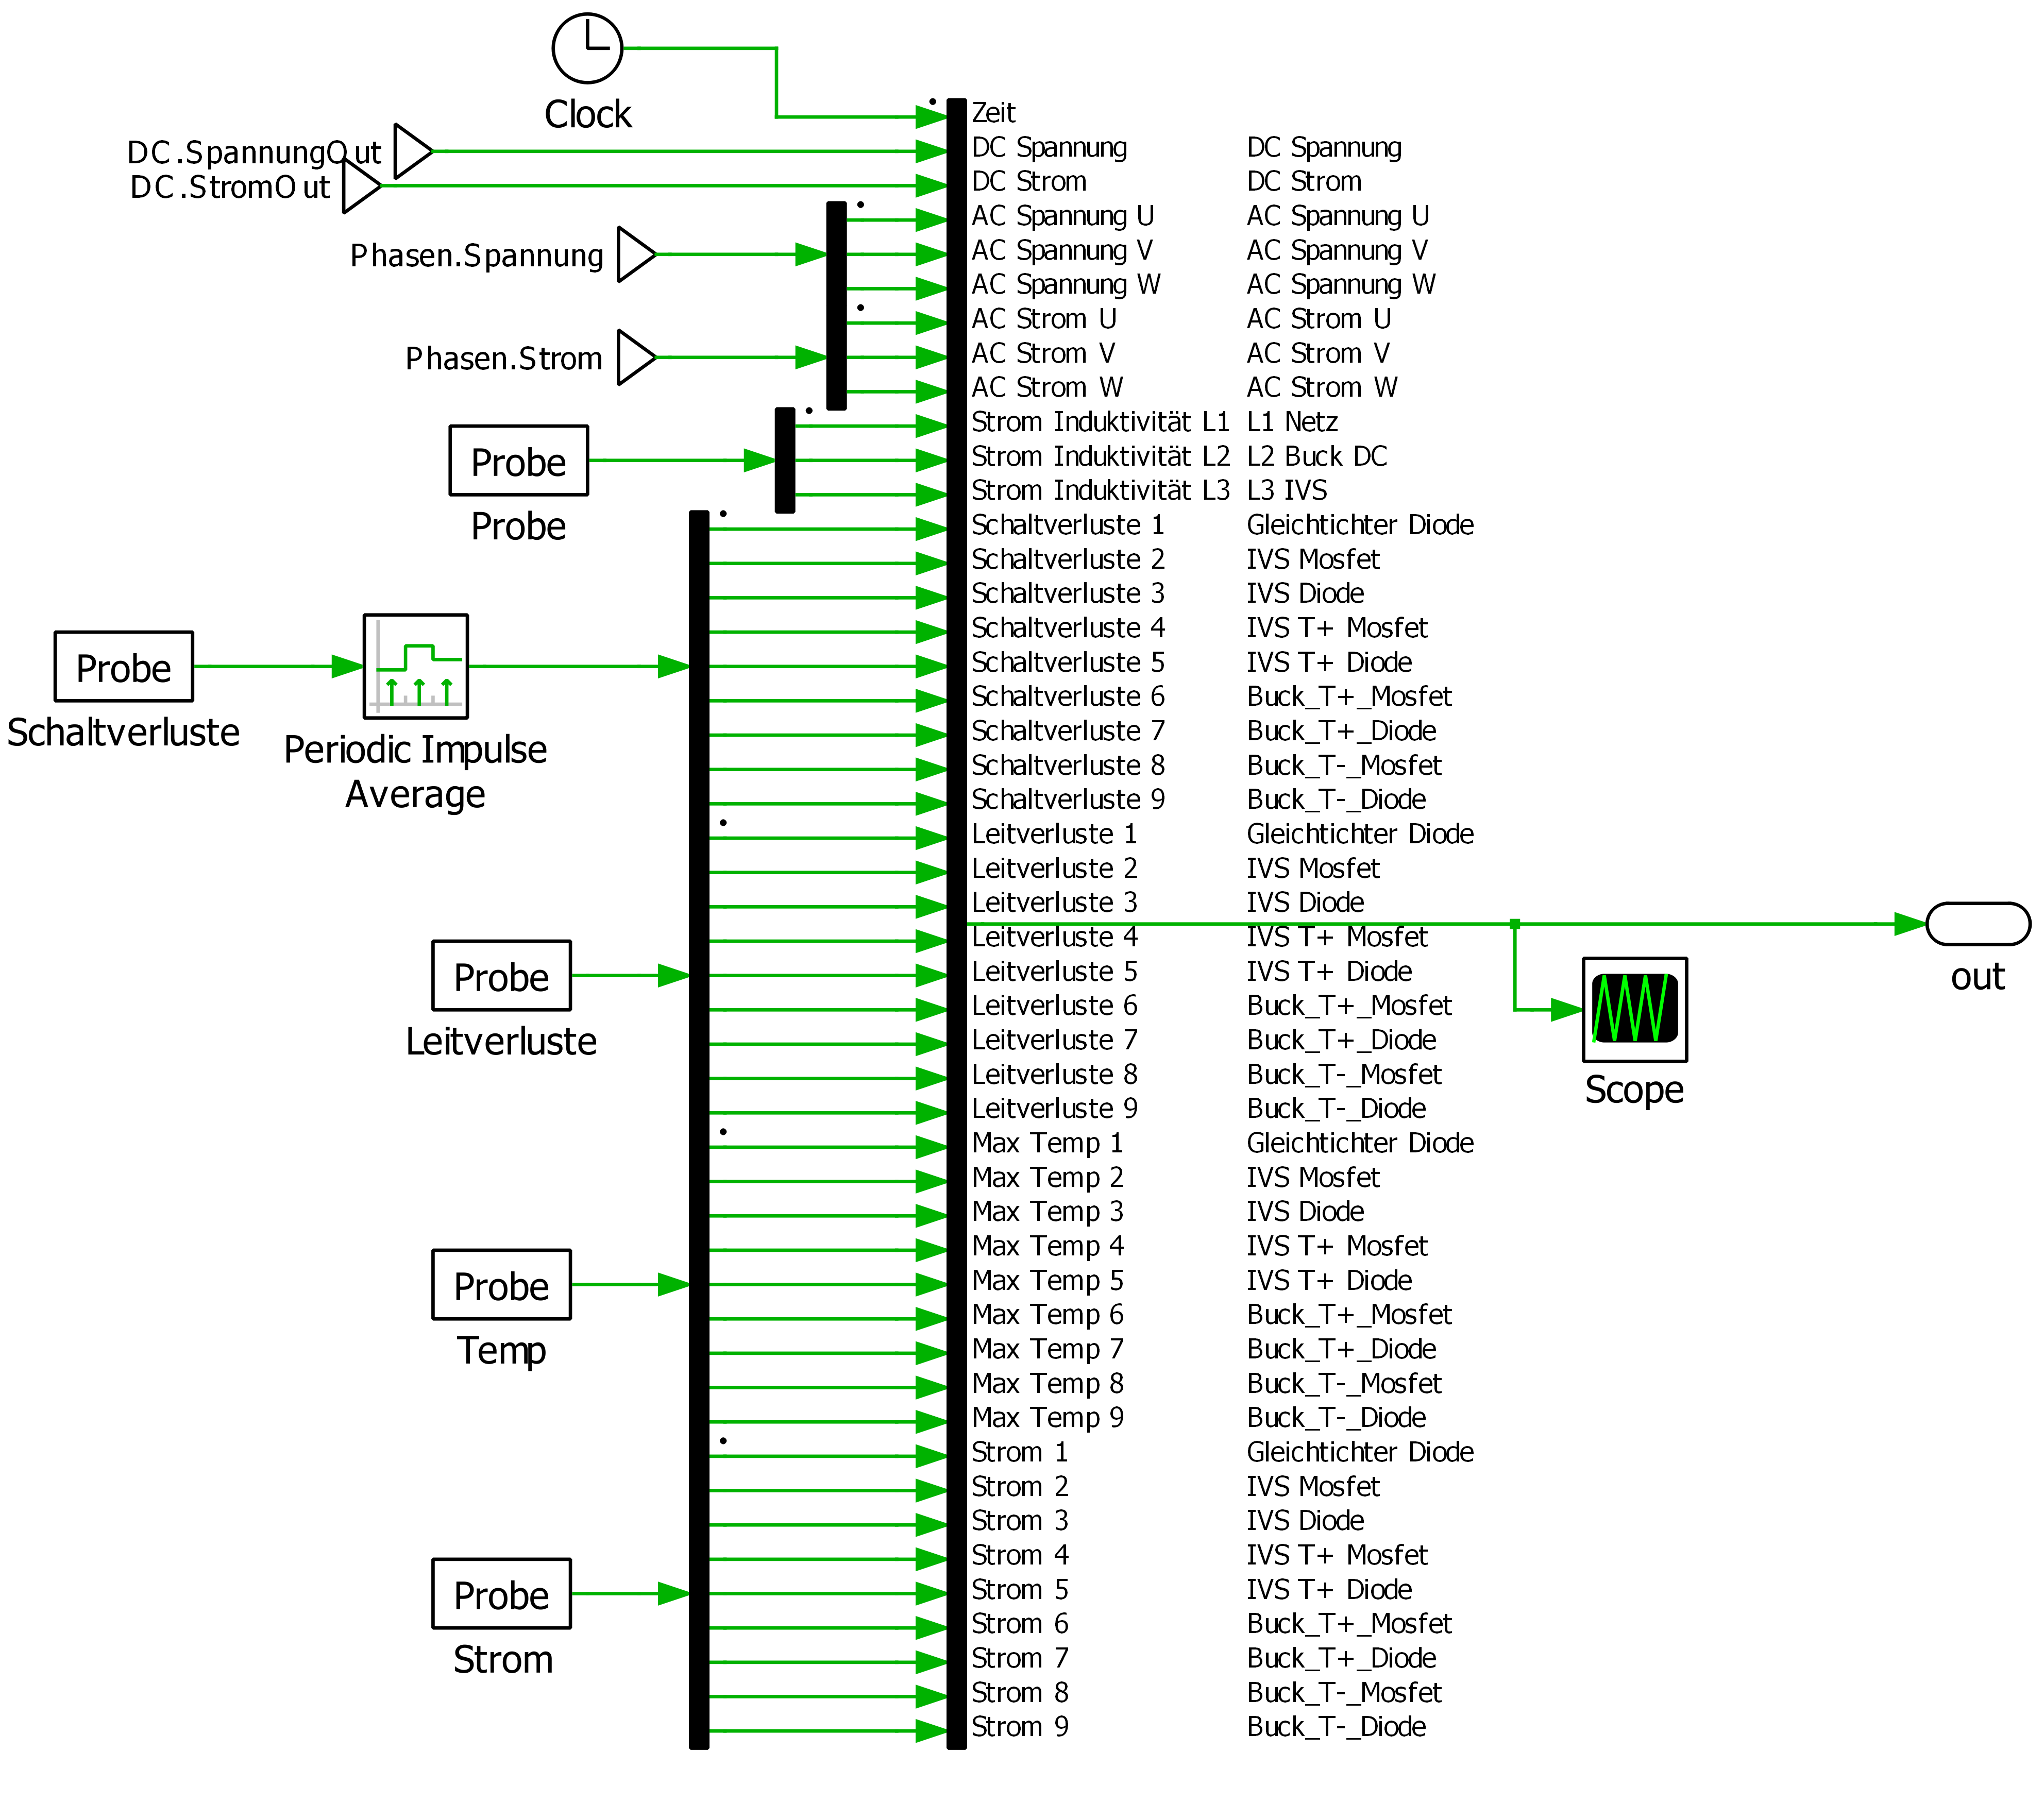
\includegraphics[width=1\linewidth]{content/Grafiken/Plecs_Out}
\caption{Zusammenfassung der Simulationsoutputs}
\label{fig:plecsout}
\end{figure}


\section{Randbedingungen}
Für den Gleichrichter werden grundlegende Parameter festgelegt, um die Auslegung für die Simulation durchführen zu können. Die Leistung von 200 kW wird als Grundlage festgelegt, da höhere Ströme aufgrund der Halbleitermodule und thermischen Belastung in einem Gerät Probleme bei der Umsetzung verursachen würden. Höhere Ströme würden die Stromtragfähigkeit gängiger Platinen übersteigen und damit die Kosten übermäßig steigern. Die Ausgangsspannung von maximal 680 V ergibt sich aufgrund der Spannungsfestigkeit der Halbleitermodule, welche 1200 V beträgt. Diese muss aufgrund von Spannungsspitzen bei Schaltvorgängen der Halbleiter weiter begrenzt werden. Aufgrund der Abschätzung der Kommutierungsinduktivität, die beim Schaltvorgang zu Überspannungen führt, welche die Lebensdauer der Halbleiter beeinträchtigen können, wird ein größerer Abstand zur Halbleiterspannung gewählt. Es wird sich für diese Spannungsklasse entschieden, da diese bereits etabliert und in breiter Masse verfügbar ist. Die Netzfrequenz sowie das Spannungsband wird anhand der Anforderungen für stationären Betrieb im deutschen Stromnetz definiert. Die Spannungsschwankung wird auf \pm 10 \% der Netznennspannung reduziert da kurzfristige Änderungen und entsprechende Kompensationen später betrachtet werden. Für die Simulation werden die in Tabelle \ref{tab:Betriebspara} aufgeführten Betriebsparameter verwendet. Die beiden Topologien werden verglichen, um die beste Lösung zu finden. Dabei wird der Einfluss der Systemdienstleistungen bei einem Phasenversatz von 0° und 30° der Eingangsströme berücksichtigt. Um die Eingangsströme bei Phasenverschiebung auszugleichen, wird die Ausgangsleistung um den Faktor cos(30°) reduziert. Die Kühlplattentemperatur von 80 °C wird aufgrund der Wahl einer Wasserkühlung für den Demonstrator gewählt.

\begin{table}
	\centering
	\caption{Auflistung der Simulationsbetriebsparameter}
	\begin{tabular}{c c}

		Ausgangsspannung \gls{Ua} & 680 V \\
		\hline
		Ausgangsleistung & 200 kW bei $\varphi = 0°$\\
		\hline
		Phasenverschiebung & 0 / 30 Grad \\
		\hline
		Kühlplattentemperatur & 80 °C \\
		\hline
		Schaltfrequenz & 20 kHz \\
		\hline
		Netzspannung \gls{Ull} & 617 \si{\volt} \\
		\hline
		Netzfrequenz &		50 Hz \\
		\hline
		Netzspannungsschwankung & 10 \% \\
	\end{tabular}
	\label{tab:Betriebspara}
\end{table}

Für die Auswertung wird der eingeschwungene Zustand des Systems betrachtet, dieser wird anhand des Temperaturverhaltens der Halbleiter kontrolliert. Dies erleichtert die Auslegung der Regler, die Parameter werden so gewählt, dass ein stabiler Zustand erreicht wird und keine Schwingungen auftreten. Außerdem wird für die Auswertung die letzte Periode der Simulation verwendet, da hier der thermische Vorgang eingeschwungen ist. Dieser Abschnitt wird für eine spätere Betrachtung gespeichert.

\section{Tiefsetzsteller}
Der Tiefsetzsteller kann entkoppelt vom Gleichrichter betrachtet werden, was für die Auslegung der Induktivität von Vorteil ist. Die Regelung kann ebenfalls entkoppelt erfolgen, sodass eine getrennte Stabilitätsbetrachtung und Optimierung möglich ist. 
	\subsection{Auslegung der Induktivität}
	Die Speicherdrossel wird nach der Formel \ref{eq:BuckL} ausgelegt, wobei die Netzspannung maximal $U_{LLmaxPeak}=1,1 \cdot 617\, \si{\V} \cdot \sqrt{2}=959,8\, \si{\V}$ und die Ausgangsspannung $U_{a,min}$ liegt bei mindestens 482 \si{\V}. Daraus ergeben sich die maximalen Parameter, die der Tiefsetzsteller realisieren muss. Es ergibt sich eine Induktivität von 134,16 \si{\micro \henry}, siehe Formel \ref{eq:BuckLwert}. Die gespeicherte Energie beträgt 7,78 Joule bei einem Ausgangsstrom von 295 A. 
	\begin{equation}
	\label{eq:BuckLwert}
	L_{T}= \dfrac{U_{LLmaxPeak}-U_{amin}}{f_{sw} \cdot \Delta I} \cdot D = \dfrac{959,8\,\si{\V} - 482\, \si{\V}}{20\, \si{\kilo \hertz}\cdot 0,3 \cdot 295\, \si{\ampere}} \cdot \dfrac{482\, \si{\V}}{959,8\, \si{\V}}= 134,16 \,\si{\micro \henry} 
	\end{equation}
	\begin{equation}
		E=\dfrac{1}{2} \cdot L_{T} \cdot I_{a}^{2} = \dfrac{1}{2} \cdot 134,16\, \si{\micro \henry}  \cdot 294\, \si{\ampere} = 7,78\, \si{\joule}
	\end{equation}
	\subsection{Regelung}
	Die Regelung kann mit den im Abschnitt \ref{sec:Buck} beschriebenen Eingangsspannungsverhältnissen ausgelegt werden. Der Tastgrad (Duty Cycle \gls{D}) ist das Verhältnis von Eingangsspannung zu Ausgangsspannung. Aufgrund der sechspulsigen Zwischenkreisspannung schwankt der Duty Cycle \gls{D} geringfügig, da eine feste Ausgangsspannung gewünscht ist, kann die Regelung mit einem PI-Regler realisiert werden.\\
	Der Tiefsetzsteller wird durch einen PI-Regler zur Fehlerkorrektur angesteuert, wobei der ideale Tastgrad aus der gewünschten Ausgangsspannung und der Zwischenkreisspannung \gls{Upn} als Vorsteuerung dient. Die gewünschte Ausgangsspannung \gls{Ua} wird durch den Sollstrom und den bekannten Lastwiderstand generiert. Der Tastgrad \gls{D} wird dann einem PWM-Generator zugeführt, der das Steuersignal mit der gewünschten Schaltfrequenz von 20 kHz erzeugt. Um die Schaltverluste und die Leitungsverluste beim Kommutieren in den Dioden zu berücksichtigen, wird eine Totzeit von 500 \si{\nano \second} eingestellt, siehe Abbildung. \ref{fig:iafbuckcontrol}.
	\begin{figure}[H]
		\centering
		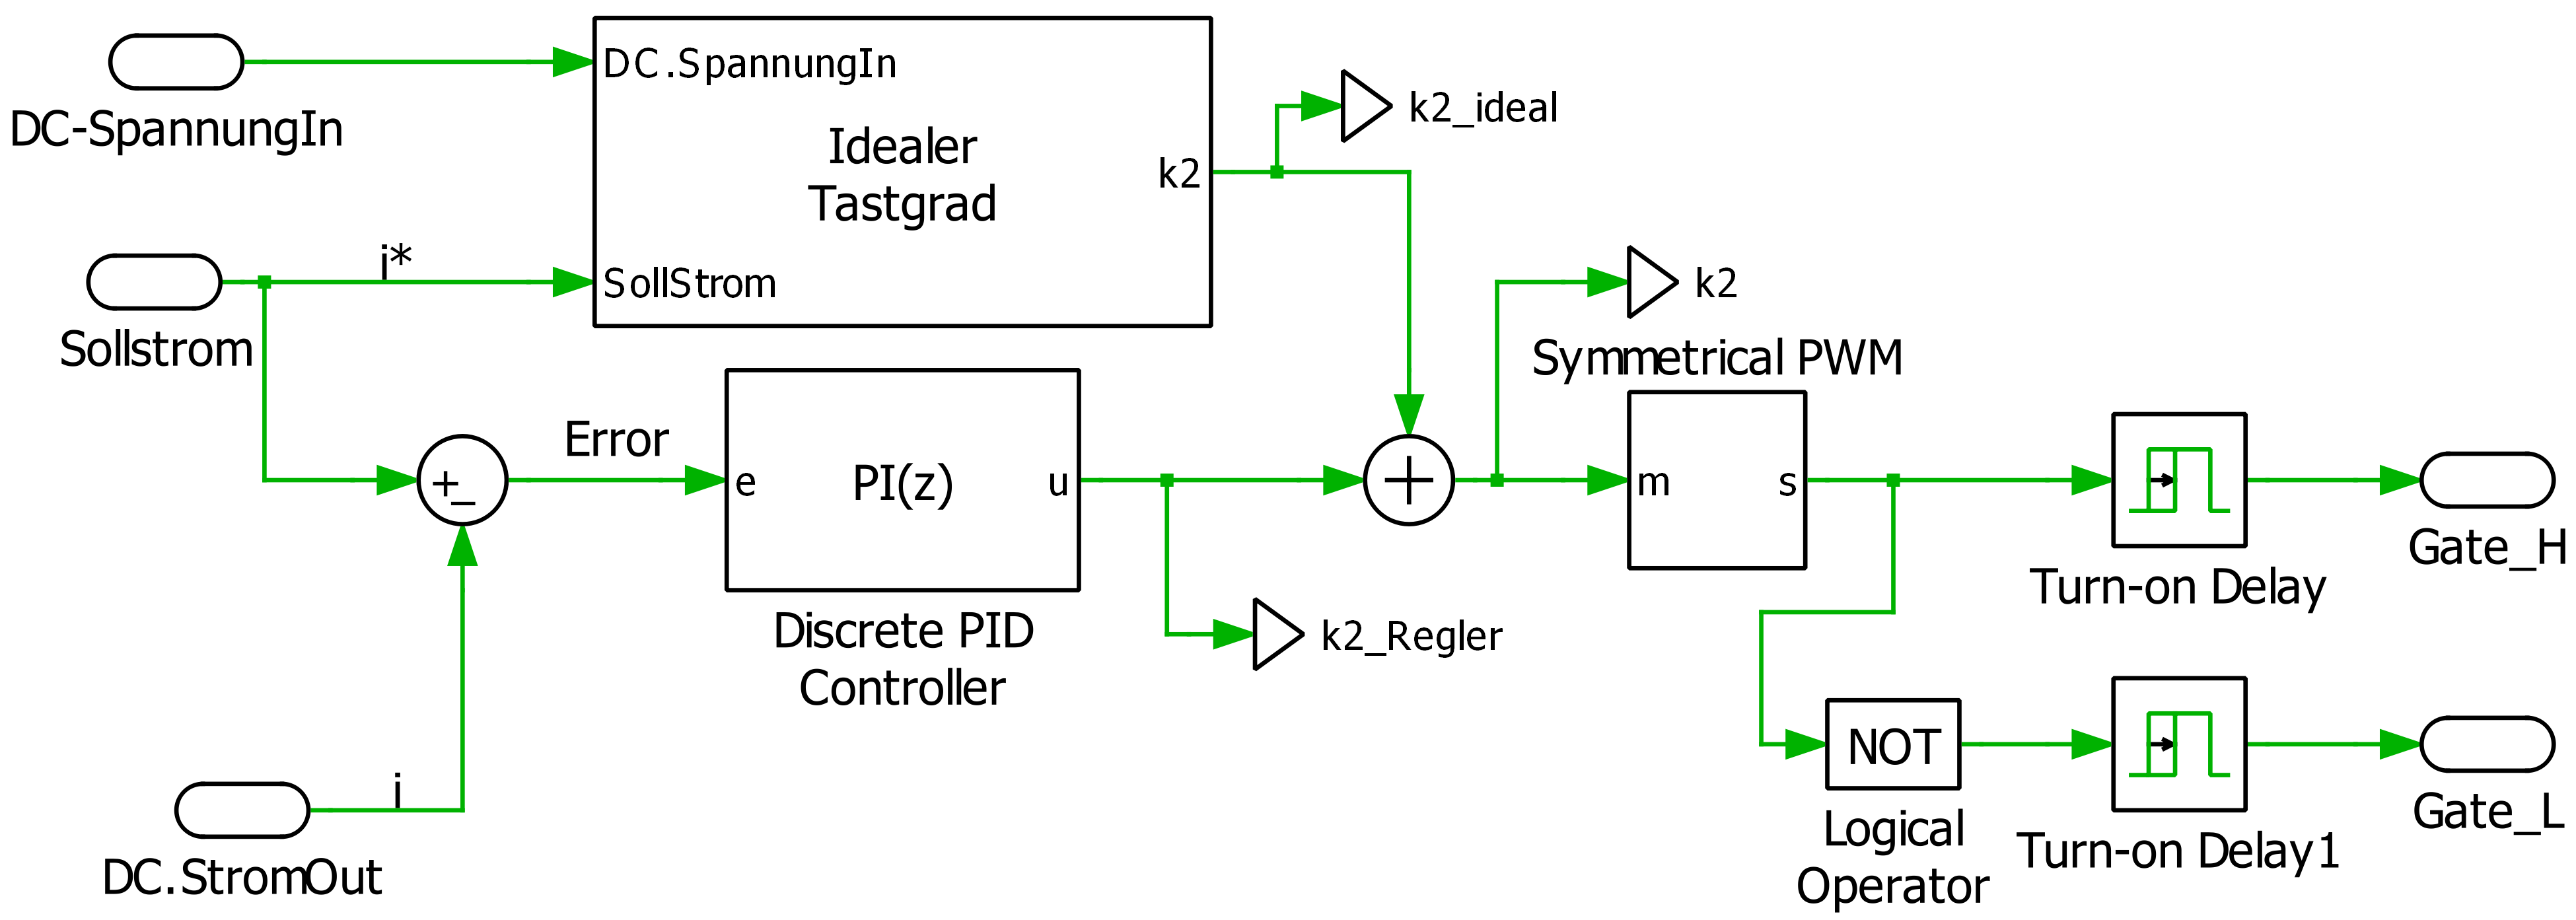
\includegraphics[width=1\linewidth]{content/Grafiken/IAF_BuckControl}
		\caption{Regelung des Tiefsetzstellers des IAF}
		\label{fig:iafbuckcontrol}
	\end{figure}


\section{IAF}
	Der Schwerpunkt der Simulation liegt auf den Leistungshalbleitern, deren Anordnung in Abbildung \ref{fig:iafplecsmain}, \ref{fig:iafplecsbuck} und \ref{fig:iafplecsivs} zu entnehmen ist. Zur Bestimmung der Verlustleistung werden Modelle von Infineon verwendet, wobei die Dioden aus dem Modul FS100R12W2T7 \cite{FS100R12W2T7} verwendet werden und für den \gls{IVS} ein Modul mit 5 \si{\milli \ohm} \gls{SiC} \gls{MOSFET} ausgewählt wird. Die Halbbrücke an der Induktivität wird aus einem Modul mit 1,4 \si{\milli \ohm} aufgebaut \cite{FF4MR12W2M1H}. Alle Halbleiter haben eine Spannungsfestigkeit von 1200 V.
	\begin{figure}
		\centering
		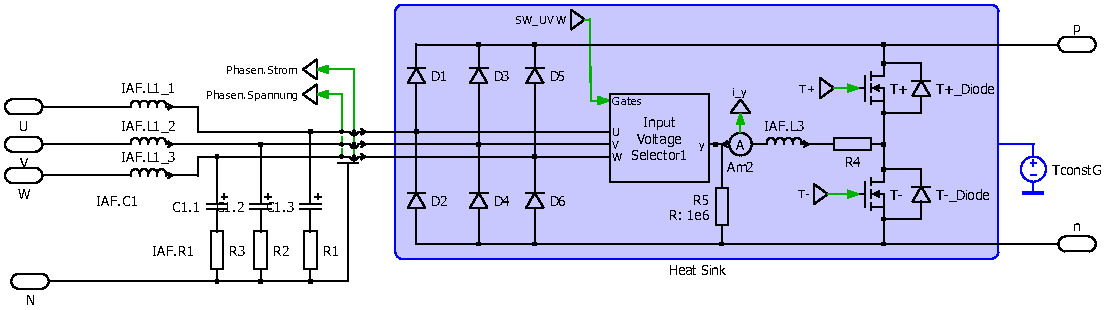
\includegraphics[width=1\linewidth]{content/Grafiken/IAF_Plecs_main}
		\caption{Simulationsaufbau der Halbleiter des IAF}
		\label{fig:iafplecsmain}
	\end{figure}
	\begin{figure}
		\centering
		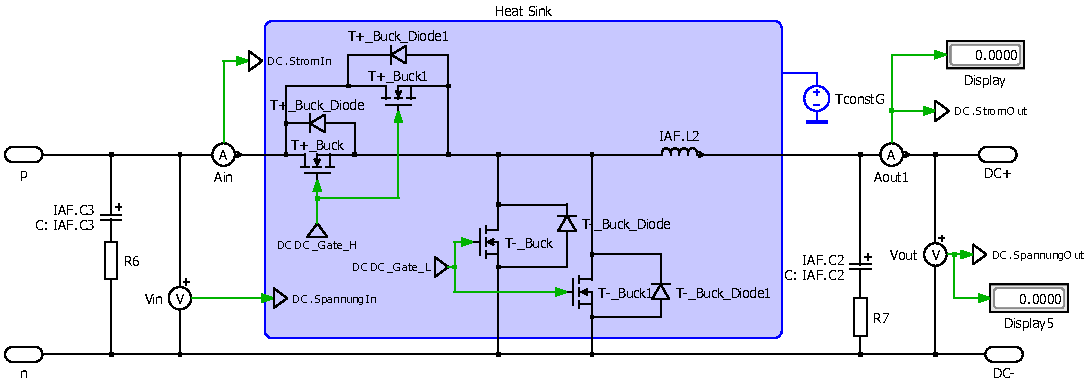
\includegraphics[width=1\linewidth]{content/Grafiken/IAF_Plecs_Buck}
		\caption{Simulationsaufbau der Halbleiter des Tiefsetzstellers vom IAF}
		\label{fig:iafplecsbuck}
	\end{figure}
	
	\begin{figure}
		\centering
		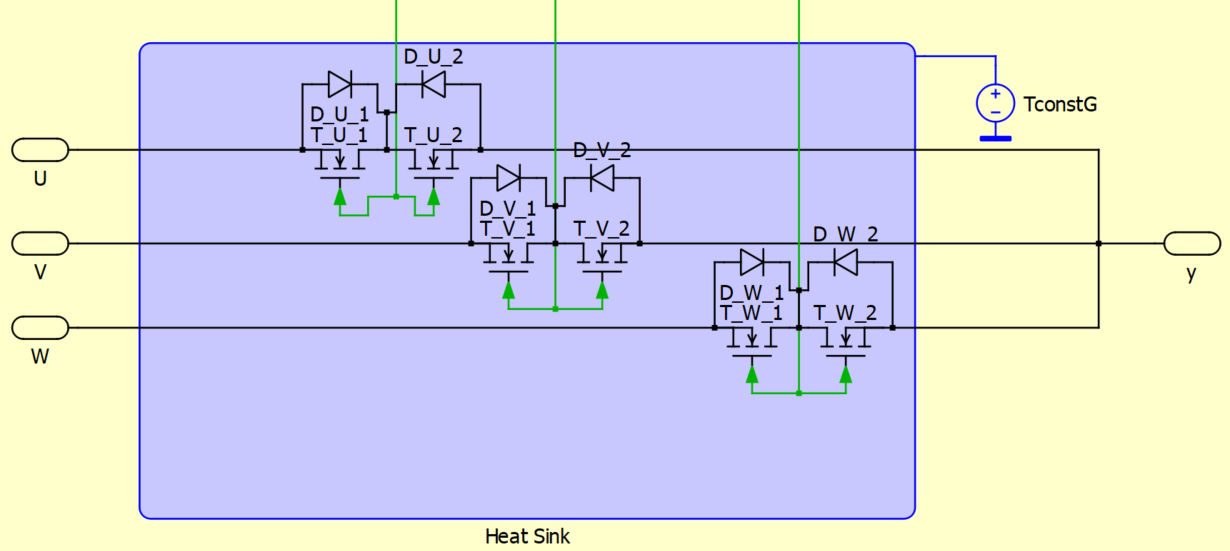
\includegraphics[width=0.7\linewidth]{content/Grafiken/IAF_Plecs_IVS}
		\caption{Simulationsaufbau der Halbleiter des IVS vom IAF}
		\label{fig:iafplecsivs}
	\end{figure}
	

	\subsection{Auslegung der Induktivitäten}
	Zur Auslegung der Induktivität wird vom Nennbetrieb ohne Phasenverschiebung ausgegangen. Dazu wird der $\hat{I}_{max}$ gebildet siehe Formel \ref{eq:Idachmax}, welcher durch Netzspannungsabfall um 10 Prozent maximal wird und somit 294,07 Ampere beträgt. Ohne Phasenverschiebung erreicht dieser bei 30 Grad der Sinuswelle sein Maximum, siehe Formel \ref{eq:IAF_I0}. Somit ergibt sich ein Spitzennennstrom $I_{IAF0°}$ von 147,04 Ampere.
	\begin{equation}
		\label{eq:Idachmax}
		\hat{I}_{max} = \dfrac{\sqrt{2} \cdot P   }{ \sqrt{3}  \cdot  U_{LLrms} \cdot 0,9} = \dfrac{\sqrt{2} \cdot 200\, \si{\kilo \watt}} { \sqrt{3} \cdot 617\, \si{V} \cdot 0,9} = 294,07\, \si{\A}
	\end{equation}
	
	\begin{equation}
		\label{eq:IAF_I0}
		I_{IAF0°}= sin(30°)\cdot \hat{I}_{max}=sin(30°)\cdot 294,07 \,A = 147,04\, \si{\A}
	\end{equation}
	
	Der Rippelstrom wird auf 30 \% des Nennstroms ausgelegt. Daher muss die Induktivität einen Wert von 272 \si{\micro \henry} haben, siehe Formel \ref{eq:Livs0}. Zur Bewertung der Induktiven Komponenten wird die gespeicherte Energie in der Drossel verwendet, diese berechnet sich nach Formel \ref{eq:EL_IVS0}
		
		\begin{equation}
			\label{eq:Livs0}
			L_{IVS0°}= \dfrac{U_{LLmaxPeak}}{4\cdot f_{sw} \cdot 0,3 \cdot I_{IAF0°}} = \dfrac{959,8\, V}{4 \cdot 20\, kHz \cdot 0,3 \cdot 147,04\, A}= 272\, \si{\micro \henry}
		\end{equation}
		
		\begin{equation}
			\label{eq:EL_IVS0}
			W_{L-IVS0°}=\dfrac{1}{2} \cdot L_{IVS} \cdot I_{IAF0°}^{2} = \dfrac{1}{2} \cdot 272\, \si{\micro \henry} \cdot (147,04\, \si{\A})^{2} =  2,94 \, \si{\joule}
		\end{equation}
		
		Bei der Betrachtung der Energie ist zu beachten, dass der Strom in der Drossel bei Blindleistung ansteigt und somit die Energie im quadratischen Verhältnis zunimmt. Bei Phasenverschiebung von 30 Grad ändert sich die Amplitude auf $sin(60°)$ und damit der Strom auf etwa 255 Ampere.
			
		
		
		\begin{equation}
			\label{eq:IAF_I30}
			I_{IAF30°}= sin(60°)\cdot \hat{I}_{max}=sin(60°)\cdot 294,07 \,A =254,68\, \si{\A}
		\end{equation}
		
		
		Die in der Drossel gespeicherte Energie, welche eine relevante Größe für die Bewertung darstellt, beträgt 8,82 Joule (siehe Formel \ref{eq:EL_IVS30}).
		
		\begin{equation}
			\label{eq:EL_IVS30}
			W_{L-IVS30}=\dfrac{1}{2} \cdot L_{IVS} \cdot I_{IAF30°}^{2} = \dfrac{1}{2}\cdot 272\, \si{\micro \henry} \cdot (254,68\, \si{\A})^{2} =  8,82 \, \si{\joule}
		\end{equation}
		
		
		
		Zusätzlich wird eingangsseitig eine Filterinduktivität $L_{IAF-N}$ mit dem Wert 1~\si{\micro \henry} eingesetzt, um das Verhalten des Netztrafos nachzubilden. Zur Bewertung der Induktiven Komponenten wird die gespeicherte Energie in der Drossel verwendet, dazu wird der Scheitelwert des Stroms $\hat{I}_{max}$ benötigt, siehe Formel \ref{eq:Idachmax}. Die Netzdrossel hat somit eine gespeicherte Energie von 0,1 Joule, siehe Formel \ref{eq:E_IAF_ACL}. Aufgrund der dreiphasigen Anwendung wird der Wert direkt mit dem Faktor 3 multipliziert.
			
			\begin{equation}
			\label{eq:E_IAF_ACL}
			W_{L-IAF-N}= 3\cdot \dfrac{1}{2} \cdot L_{IAF-N} \cdot (\hat{I}_{max})^2=\dfrac{3}{2} \cdot 1\, \si{\micro \henry} \cdot (294,07 \, \si{\ampere})^{2} = 0,13 \, \si{\joule}
		\end{equation}
	
	\subsection{Regelung}
		Die Regelung des Stroms des IVS wird anhand der Struktur von Soeiro et al. umgesetzt (vgl. Abb. \ref{fig:iafpapercontrol}) \cite{Soeiro.2013}.
		 \begin{figure}[H]
			\centering
			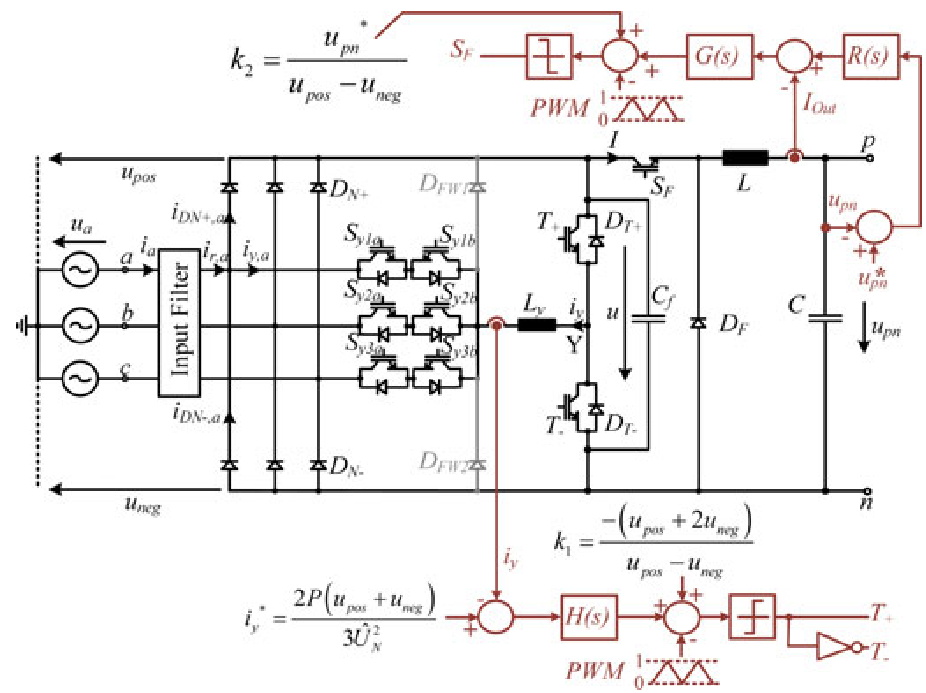
\includegraphics[width=0.8\linewidth]{content/Grafiken/IAF_Paper_Control}
			\caption{Struktur der Regelung des IAF \cite{Soeiro.2013}}
			\label{fig:iafpapercontrol}
		\end{figure}
		Die Umschaltung zwischen den Phasen erfolgt mithilfe einer vorhandenen PLL in PLECS zur Winkelbestimmung und anschließenden Sektorbestimmung. Die Sektorenzuweisung wird anhand des Phasenwinkels nach dem Schema aus Abbildung \ref{fig:b6iafsectors} umgesetzt. Die Auswahl der entsprechenden Schalter ist durch ein C-Skript implementiert (siehe Abbildung \ref{fig:plecsiafivscontrol}). 
		\begin{figure}[H]
			\centering
			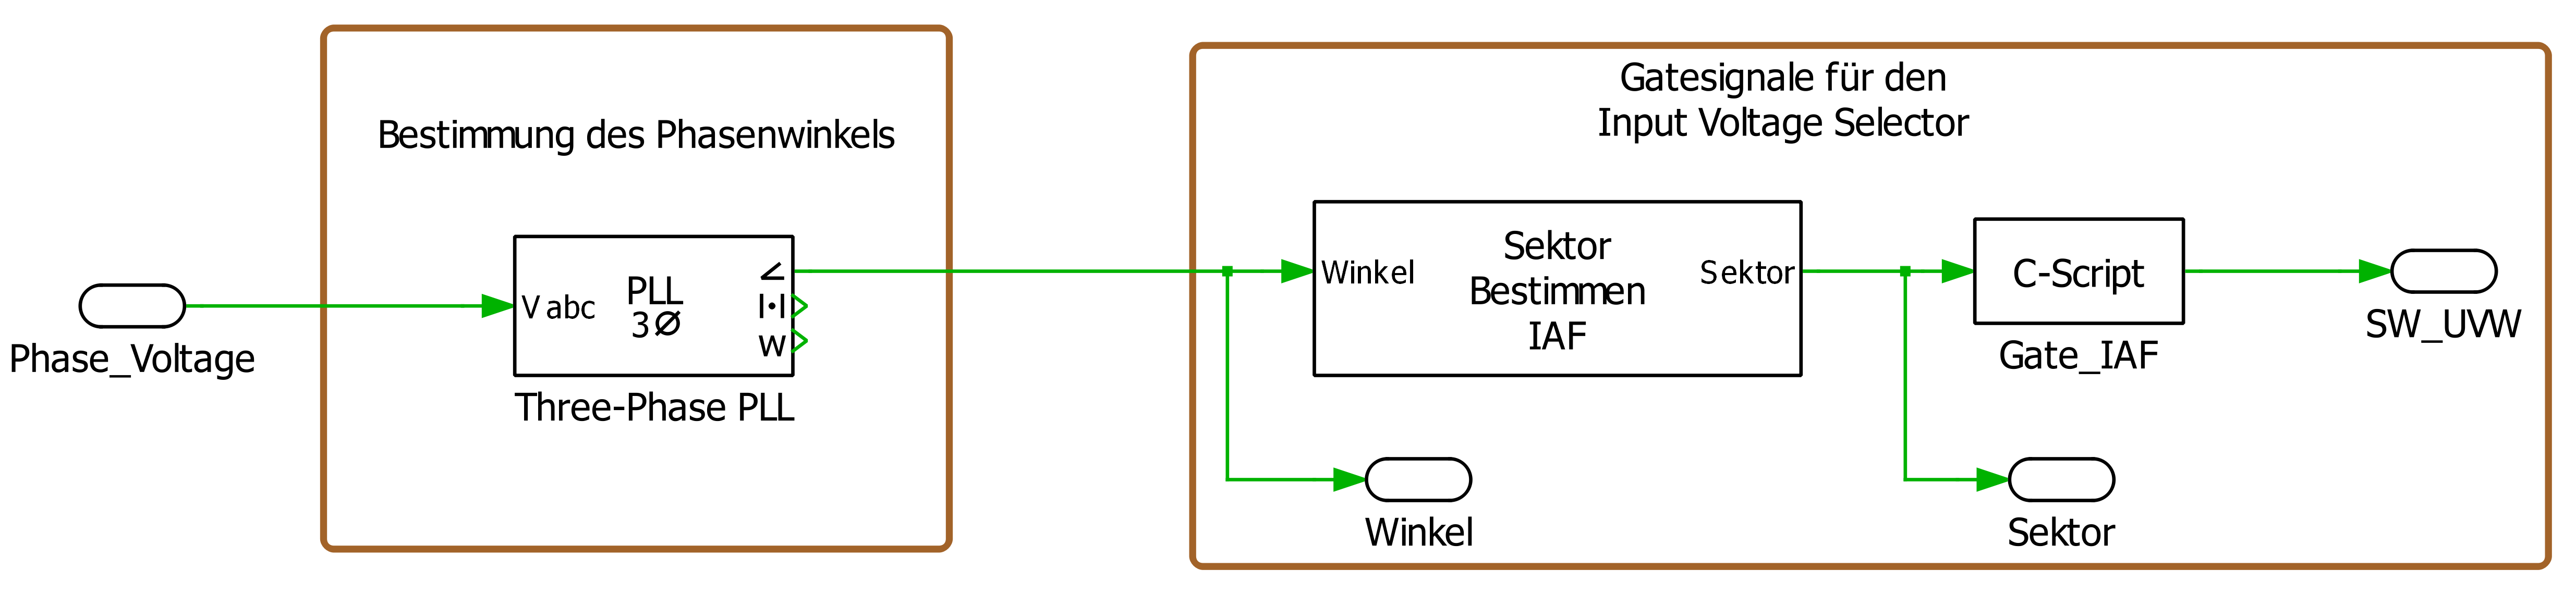
\includegraphics[width=1\linewidth]{content/Grafiken/PlecsIAFivscontrol}
			\caption{PLECS Aufbau der \gls{IVS} Ansteuerung}
			\label{fig:plecsiafivscontrol}
		\end{figure}
			Der Strom in der Drossel wird durch den idealen Stromverlauf der mittleren Phase bestimmt. Der aktuelle Phasenwinkel der Spannung wird dazu durch die PLL erfasst und kann mit einer einstellbaren Phasenverschiebung verändert werden. Die Stromamplitude \gls{I^} wird über die Netzspannung und die gewünschte Ausgangsleistung bestimmt (siehe Formel \ref{eq:IdachTheory}). Der sinusförmige Strom wird durch die Amplitude und den entsprechenden Winkel mit jeweils 120° bzw. $\dfrac{2}{3}\pi$ Phasenversatz gebildet, siehe Abb. \ref{fig:plecsiafidealephasenstrome}. Die mittlere Phase wird über die Sektorenzuweisung ausgewählt, siehe Abbildung \ref{fig:plecsiafiy}.
			\begin{equation}
				\label{eq:IdachTheory}
				\hat{I} = \dfrac{\sqrt{2} \cdot P   }{ \sqrt{3} \cdot cos(\varphi) \cdot  U_{LLrms} } 
			\end{equation}
		\begin{figure}[H]
			\centering
			\includegraphics[width=1\linewidth]{content/Grafiken/PLECS_IAF_idealePhasenströme}
			\caption{Generierung der idealen Phasenströme}
			\label{fig:plecsiafidealephasenstrome}
		\end{figure}
		
		
		\begin{figure}[H]
			\centering
			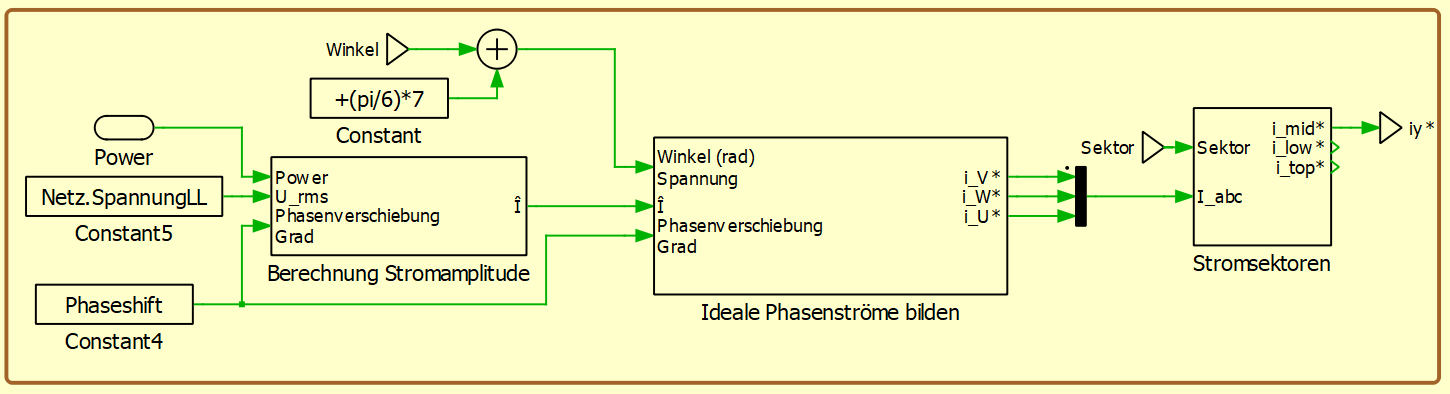
\includegraphics[width=1\linewidth]{content/Grafiken/PlecsIAFiy}
			\caption{Bestimmung des Sollstroms der mittleren Phase}
			\label{fig:plecsiafiy}
		\end{figure}
		
	Der ideale Tastgrad K1 für den Strom in der Drossel wird über das Verhältnis der Spannungen durch den formelmäßigen Zusammenhang in Gleichung \ref{eq:K1} bestimmt. 
	\begin{equation}
		\label{eq:K1}
		K1 = \dfrac{U_{mid}- U_{low}}{U_{high} -U_{low}} 
	\end{equation}
Die Stromregelung erfolgt mithilfe eines diskreten PI-Reglerblocks aus der PLECS-Bibliothek. Die Signale zur Gate-Ansteuerung werden durch einen PWM-Generator erzeugt und anschließend durch eine Einschaltverzögerung zur Totzeit-Implementierung verzögert. Dieser Aufbau ist in Abbildung \ref{fig:plecsiafivsk1} dargestellt. 
		\begin{figure}
			\centering
			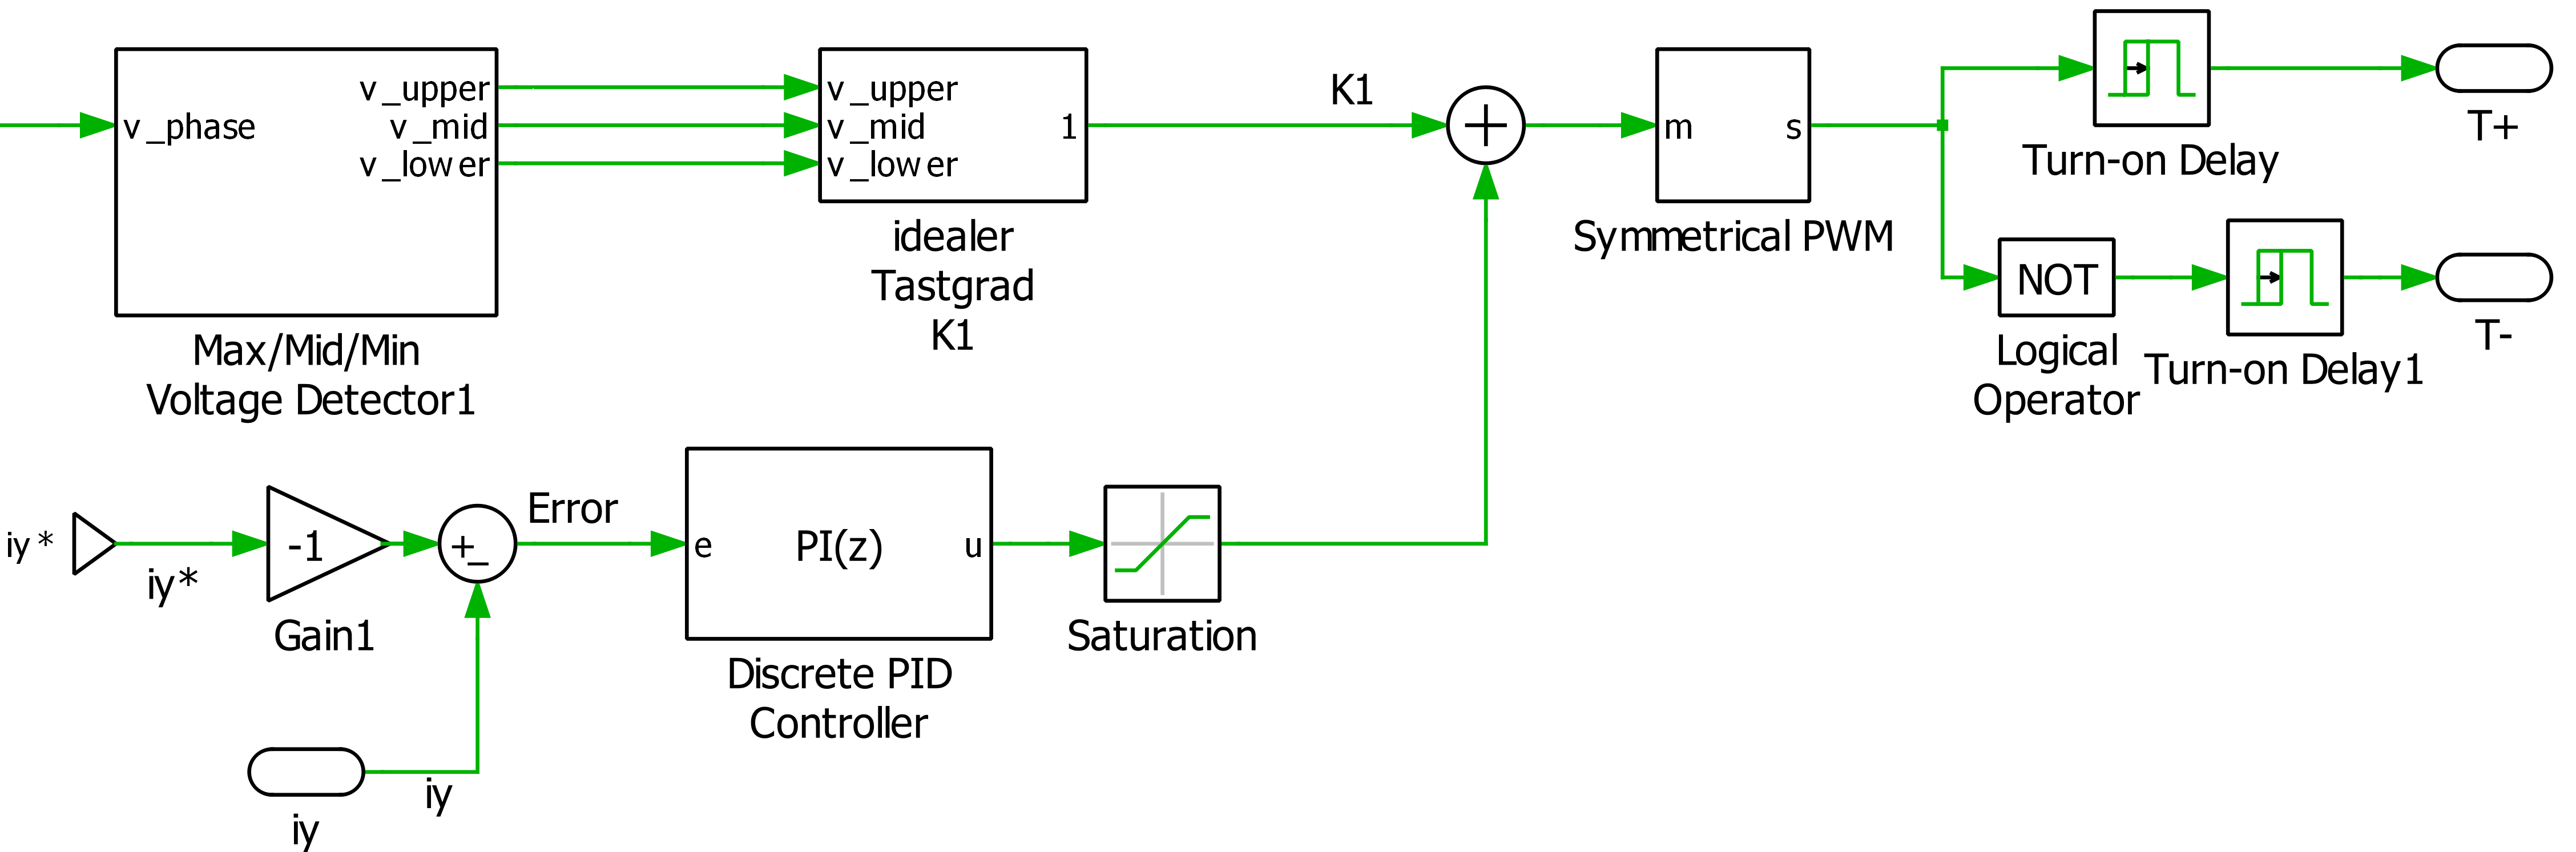
\includegraphics[width=1\linewidth]{content/Grafiken/PlecsIAFivsK1}
			\caption{Regelung des Stroms in der mittleren Phase}
			\label{fig:plecsiafivsk1}
		\end{figure}
		
		\subsection{Ergebnisse}
		Für die Auswertung werden die Simulationen für eine Dauer von bis zu zehn Sekunden durchgeführt, da zu diesem Zeitpunkt ein eingeschwungener Zustand erreicht ist. Wie in Abbildung \ref{fig:iaftemp0} zu erkennen ist, ist die Kühlplattentemperatur als Startpunkt auf 80~°C festgelegt. Die Temperatur der Dioden des Gleichrichters, welche den Hauptstrom führen, sind in grün dargestellt und ändern sich nur minimal aufgrund der Blindleistungsbereitstellung, siehe Abbildung \ref{fig:iaftemp30}. Die Temperatur beträgt knapp über 120~°C und liegt somit unterhalb der erlaubten Maximaltemperatur von 175~°C \cite{IFAGFF2}. Die Temperatur der T+/- Halbbrücke wird in Pink dargestellt und steigt bei Blindleistungsbereitstellung auf knapp 160~°C und bietet damit 15~°C Abstand zur zulässigen Maximaltemperatur.  Diese hohe Temperatur führt zwar nicht zu einem direkten Ausfall der Halbleiter, hat aber einen starken Einfluss auf die Lebensdauererwartung. Die Anzahl der Temperaturzyklen bei Temperaturen über 150~°C führt zu einem wahrscheinlichen Ausfall bei weniger als 10~000 Zyklen \cite{SicTemp}. Daher sollte eine Erhöhung der Chipfläche für die Halbbrücke am \gls{IVS} überlegt werden. Die Temperatur des Tiefsetzstellers wird in Rot dargestellt und sinkt aufgrund der reduzierten Ausgangsleistung bei Blindleistungsbereitstellung.  
		\begin{figure} 
			\centering
			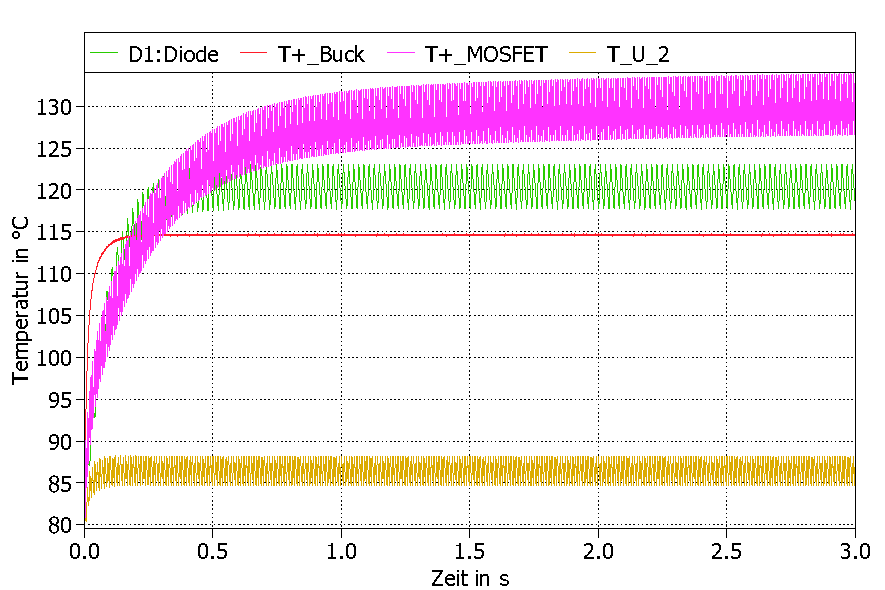
\includegraphics[width=0.9\linewidth]{content/Grafiken/IAF_Temp_0Grad}
			
			
			\caption{Temperaturverhalten der Halbleiter des IAF ohne Phasenverschiebung}
			\label{fig:iaftemp0}
		\end{figure}
		
		\begin{figure} 
			\centering
			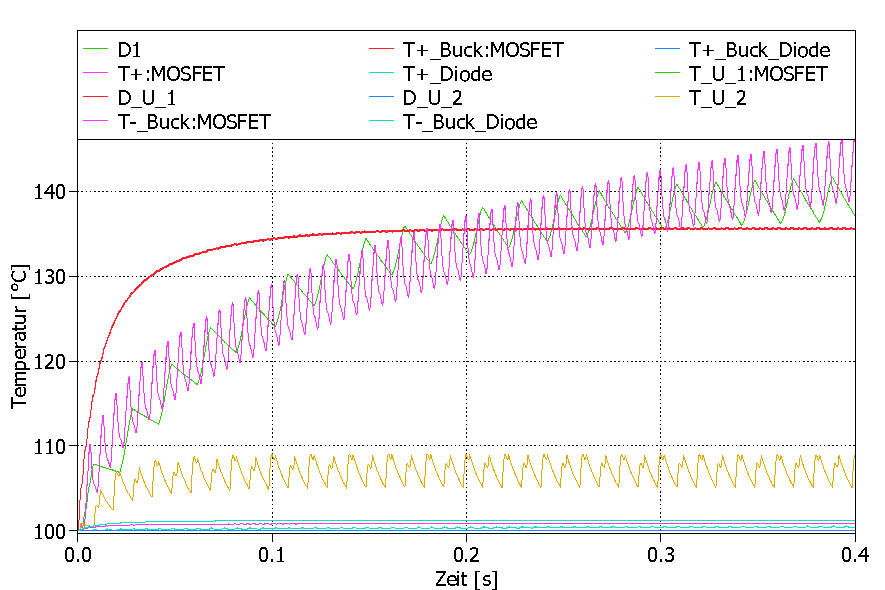
\includegraphics[width=0.9\linewidth]{content/Grafiken/IAF_Temp_30Grad}
			\caption{Temperaturverhalten der Halbleiter des IAF mit  Phasenverschiebung}
			\label{fig:iaftemp30}
		\end{figure}
		
		Die Simulationsergebnisse zeigen den erwarteten Strom- und Spannungsverlauf für die \gls{IVS} Induktivität mit einer Dreiecksform, siehe Abbildung. \ref{fig:iafacl}. Zusätzlich ist dem Eingangsstrom ein hochfrequenter Anteil überlagert, der durch die Schaltfrequenz des Tiefsetzstellers erklärt werden kann. Beim Schaltvorgang des \gls{IVS} treten starke Sprünge im Stromverlauf auf, da der Strom in der Induktivität zwischen den Phasen wechselt. Aufgrund der Eigenschaft der Spule, den gespeicherten Stromfluss aufrecht erhalten zu wollen, führt dies zu Sprüngen im Stromverlauf, da die Phasenströme zu diesem Zeitpunkt unterschiedlich sind und die Schaltvorgänge durch Totzeiten verzögert werden. Der Schaltpunkt liegt beim Maximum des Stromes in der Induktivität.\\
		In Abb. \ref{fig:iafacl30grad} wird dieses Problem durch den höheren Strom welcher in der Drossel des \gls{IVS} Pfades gespeichert und umgeschaltet werden muss noch verstärkt. Außerdem wird dadurch mehr Verlustleistung erzeugt. Dies ist auch in der Temperaturkurve in Abb. \ref{fig:iaftemp30} dargestellt. Es werden nur die höchsten Temperaturen dargestellt, dies sind die Eingangsdioden, beispielhaft an D1 in grün dargestellt sowie die \gls{MOSFET}s des T+ in pink (der Halbbrücke am \gls{IVS}), der \gls{IVS} in Gelb sowie des Tiefsetzstellers in rot. Ohne Blindleistung ist die Temperatur des IVS unter 90~°C und steigt durch den höheren Strom aufgrund der Phasenverschiebung um über 20~°C. Um den Sinusverlauf im Mittel besser erkennen zu können, ist in Abbildung \ref{fig:iafacl30grad} der Stromverlauf nach einer Tiefpassfilterung für die Schaltfrequenzanteile dargestellt. Dadurch ist die Phasenverschiebung besser ersichtlich, siehe Verlauf A Filter.
		\begin{figure}
			\centering
			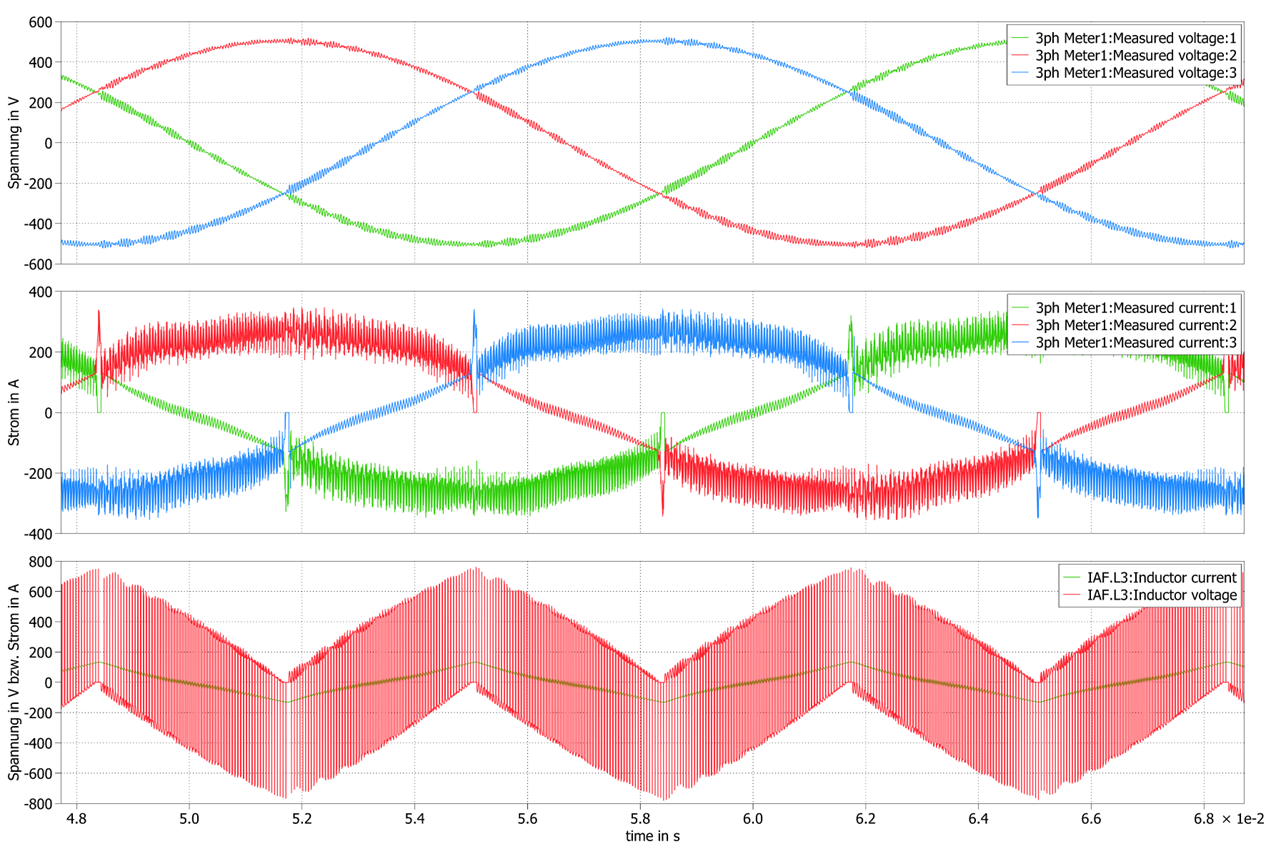
\includegraphics[width=1\linewidth]{content/Grafiken/IAF_AC+L}
			\caption{Simulationsergebnisse des IAF ohne Phasenverschiebung, Eingangsspannung und Ströme, Strom in der IVS Induktivität }
			\label{fig:iafacl}
		\end{figure}
		\begin{figure}
			\centering
			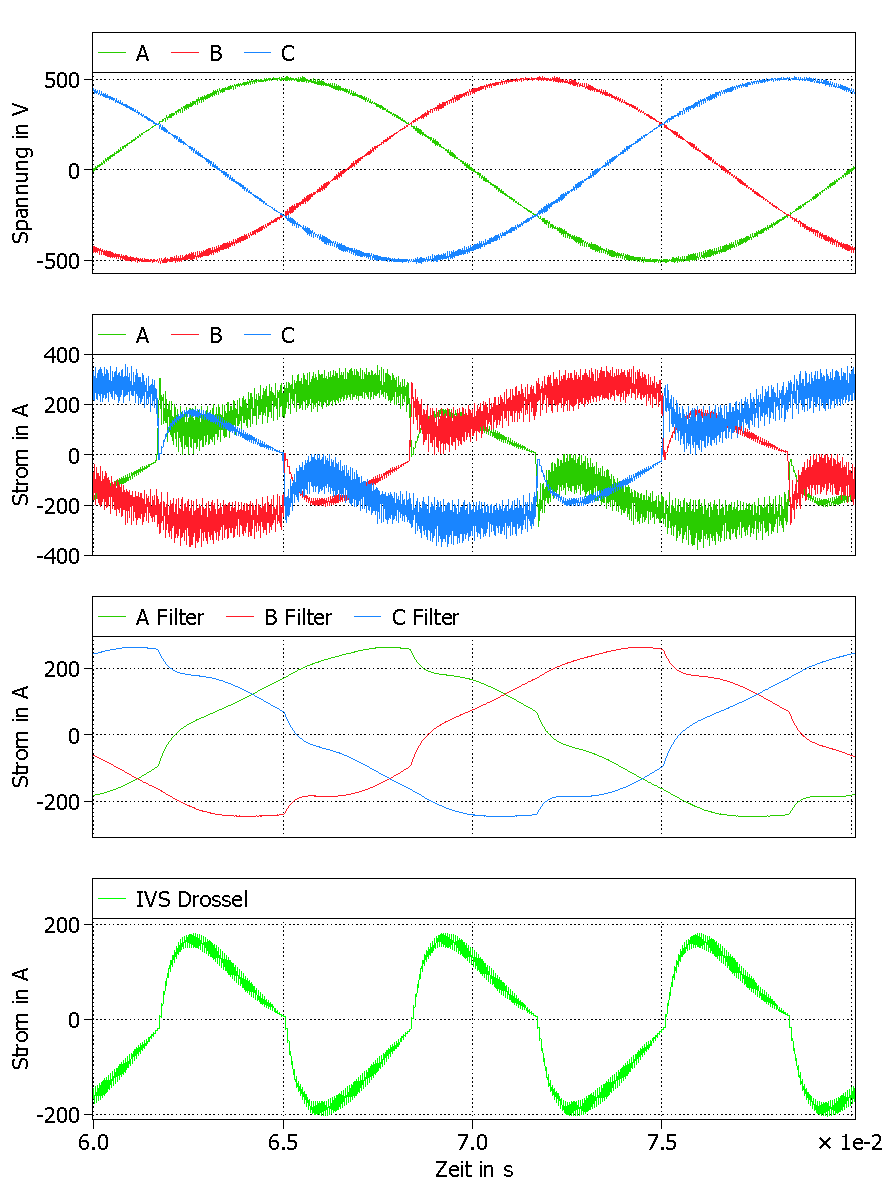
\includegraphics[width=1\linewidth]{content/Grafiken/IAF_AC+L_30Grad}
			\caption{Simulationsergebnisse des IAF bei 30 Grad Phasenverschiebung, Eingangsspannung und Ströme, Strom in der IVS Induktivität }
			\label{fig:iafacl30grad}
		\end{figure}
		Die Topologie hat aufgrund der Anforderung an Blindleistungsbereitstellung einen Nachteil durch den IVS, da dieser sprunghafte Änderungen des Stromverlaufs verursacht. Diese starken Sprünge führen dazu, dass die THD des Stroms deutlich verschlechtert wird. Die THD liegt bereits ohne Phasenverschiebung bei etwa 15~\%, und mit Phasenverschiebung verdoppelt sich dieser Wert auf etwa 32 \%. Dies ist proportional zum vom \gls{IVS} geschalteten Drosselstrom, der sich ebenfalls etwa verdoppelt.  Somit kann der IAF den Anforderungen nur schwer gerecht werden, da weitere Filterstufen benötigt würden. Dies lässt sich auch gut anhand der Arbeit von Schrittwieser et al. sehen, welche den SWISS und \gls{IAF} mit 8~kW Leistung beschreibt. Bei ihrem Prototyp macht der EMI-Filter knapp 5\% mehr des Volumens aus als beim SWISS Rectifier \cite{IAF99}.
		
	

\section{B6-1/3-PWM PFC Buck}
Die in Kapitel \ref{sec:GrundlagenB6} beschriebene Schaltung wird mit insgesamt drei Halbbrückenmodulen der Firma Infineon realisiert, siehe Abb. \ref{fig:plecsb6}. Es handelt sich dabei um weit verbreitete 1200 \si{\volt} Module FF2MR12W3M1H, die einen nominellen Einschaltwiderstand von 2 \si{\milli \ohm} haben und Spitzenströme bis zu 800 \si{\ampere} schalten können \cite{IFAGFF2}.
\begin{figure}[H]
	\centering
	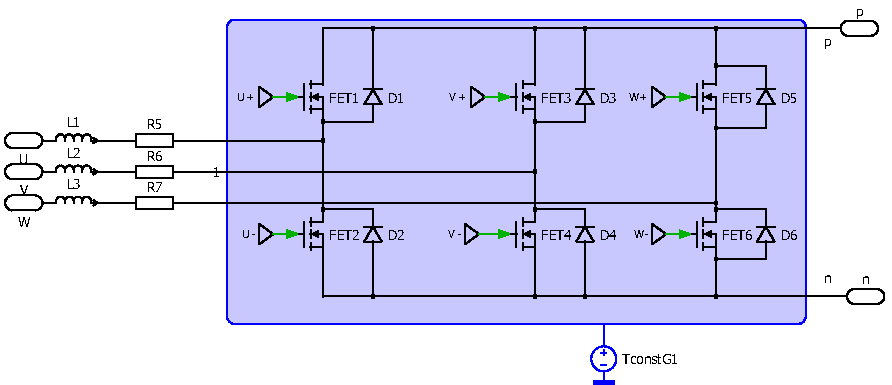
\includegraphics[width=1\linewidth]{content/Grafiken/PLECS_B6}
	\caption{PLECS Aufbau der B6 Leistungshalbleiter}
	\label{fig:plecsb6}
\end{figure}
 Um den gewünschten Ausgangsstrom bereitzustellen zu können sind für den Tiefsetzsteller zwei Halbbrückenmodule vorgesehen. Die Schaltung ist in Abbildung \ref{fig:plecsb6buck} zu finden. Es ist erkennbar, dass der Tiefsetzsteller durch den Kondensatoren C4 am Eingang des Tiefsetzstellers entkoppelt ist.
 \begin{figure}[H]
 	\centering
 	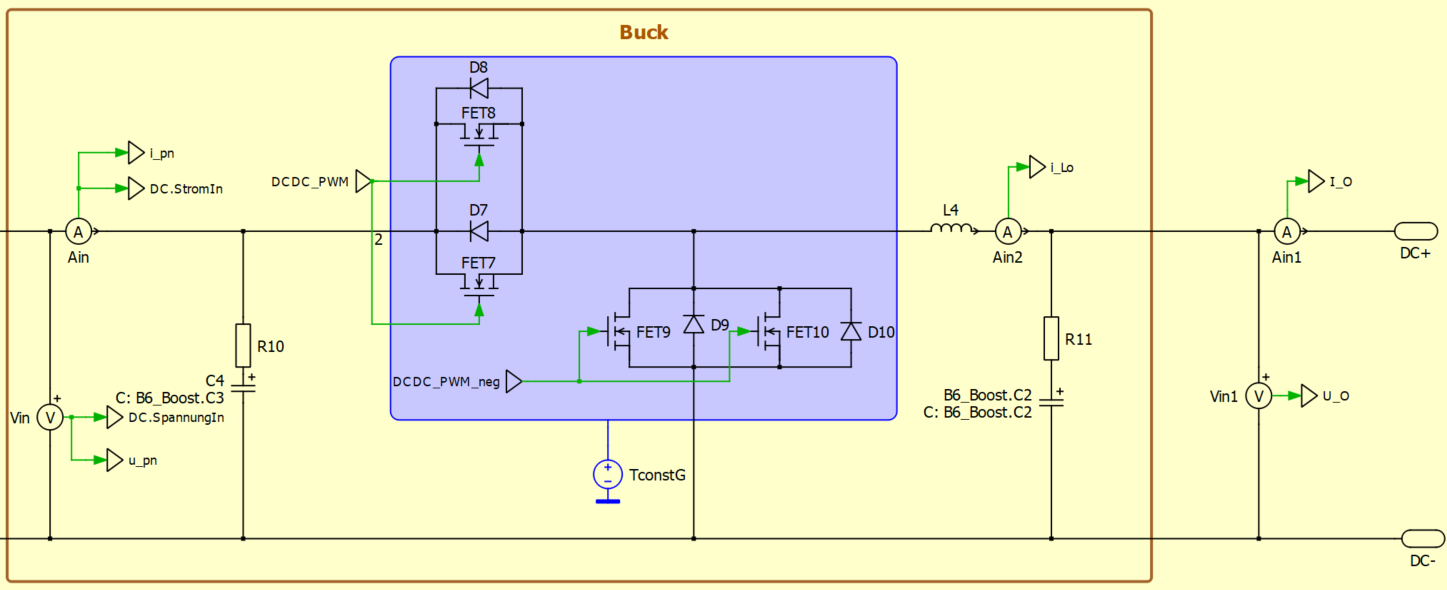
\includegraphics[width=0.9\linewidth]{content/Grafiken/PLECS_B6Buck}
 	\caption{PLECS Aufbau des Tiefsetzstellers der B6 Topologie}
 	\label{fig:plecsb6buck}
 \end{figure}
 

		\subsection{Auslegung der Netzinduktivität}
				Die Eingangsdrossel wird für den Normalbetrieb ausgelegt. Daher muss im Falle von Blindleistung die Wirkleistung reduziert werden. Wie bereits in Abschnitt \ref{sec:AnfStromnetz} erläutert, ist dies vom Netzbetreiber gestattet. Der Rippelstrom in der Drossel wird wie zuvor auf 30 \% der Grundschwingung ausgelegt, siehe Formel \ref{eq:Idachmax}. Der Rippelstrom beträgt somit 88,2 Ampere, siehe Formel \ref{eq:DeltaI_B6}.\\
			
			\begin{equation}
				\label{eq:DeltaI_B6}
				I_{\Delta max B6}= 0,3 \cdot \hat{I}_{max}= 0,3 \cdot 294,07\, \si{\A} = 88,2\, \si{\A}
			\end{equation}
			Die Induktivität kann nach der gleichen Beziehung wie für den \gls{IAF}-\gls{IVS} berechnet werden und beträgt 136 \si{\micro \henry}, siehe Formel \ref{eq:L_B6}.
			\begin{equation}
				\label{eq:L_B6}
				L_{B6}= \dfrac{U_{LLmaxPeak}}{4\cdot f{sw} \cdot I_{\Delta max B6}} = \dfrac{959,8\, \si{\volt}}{4 \cdot 20\, \si{\kilo \hertz} \cdot 88,2\, \si{\ampere}} =136\, \si{\micro \henry}
			\end{equation}
			Die in der Induktivität gespeicherte Energie wird ebenfalls durch den Zusammenhang zwischen Netzspannung und Ausgangsleistung definiert, erhöht sich jedoch nicht durch die Bereitstellung von Blindleistung. Die gespeicherte Energie pro Phase beträgt 5,88 Joule nach Formel \ref{eq:EL_B6} und muss aufgrund der dreiphasigen Ausführung mit dem Faktor drei multipliziert werden. Somit ergibt sich eine Gesamtenergie von 17,64 Joule für die Netzinduktivität der Topologie.
			
			\begin{equation}
			\label{eq:EL_B6}
			W_{LB6}= 3 \cdot \dfrac{1}{2} \cdot L_{B6} \cdot (\hat{I}_{max})^{2}= \dfrac{3}{2} \cdot 136 \,\si{\micro \henry} \cdot (294,07\, \si{\A})^{2} = 17,64 \, \si{\milli \joule}
			\end{equation}
		\subsection{Regelung}
			Die Regelung besteht aus einer vierstufigen Kaskadenstruktur, siehe Abbildung \ref{fig:b6-control-orig} (groß im Anhang \ref{fig:b6regelung}). Die erste Stufe ist die Ausgangsspannungsregelung, die aus Sollleistung und Netzspannung die gewünschte äquivalente Phasenimpedanz als Eingangsgröße für die Phasenstromregelung bildet. Die drei Regler für die Phasenströme bilden die zweite Stufe.\\
			In der dritten Stufe wird die Phase mit der mittleren Spannung ausgewählt und anhand der Phasenlage die Zwischenkreisspannung \gls{Upn} bestimmt. Die Zwischenkreisspannung ergibt sich als Sechspulsige-Gleichspannung und dient als Eingangsspannung für den Tiefsetzsteller. Die mittlere Phasenspannung wird als Referenz für den Tastgrad der entsprechenden Halbbrücke verwendet und prägt somit einen spannungsproportionalen Strom ein. Somit ist immer nur eine der drei Halbbrücken getaktet geschaltet, die anderen beiden sind wie bei einem Diodengleichrichter auf die jeweils positivste und negativste Spannung geschaltet. Die vierte Stufe ist der Tiefsetzsteller mit Reglern für den Eingangsstrom und die Ausgangsspannung.
				
			\begin{figure}
			\centering
			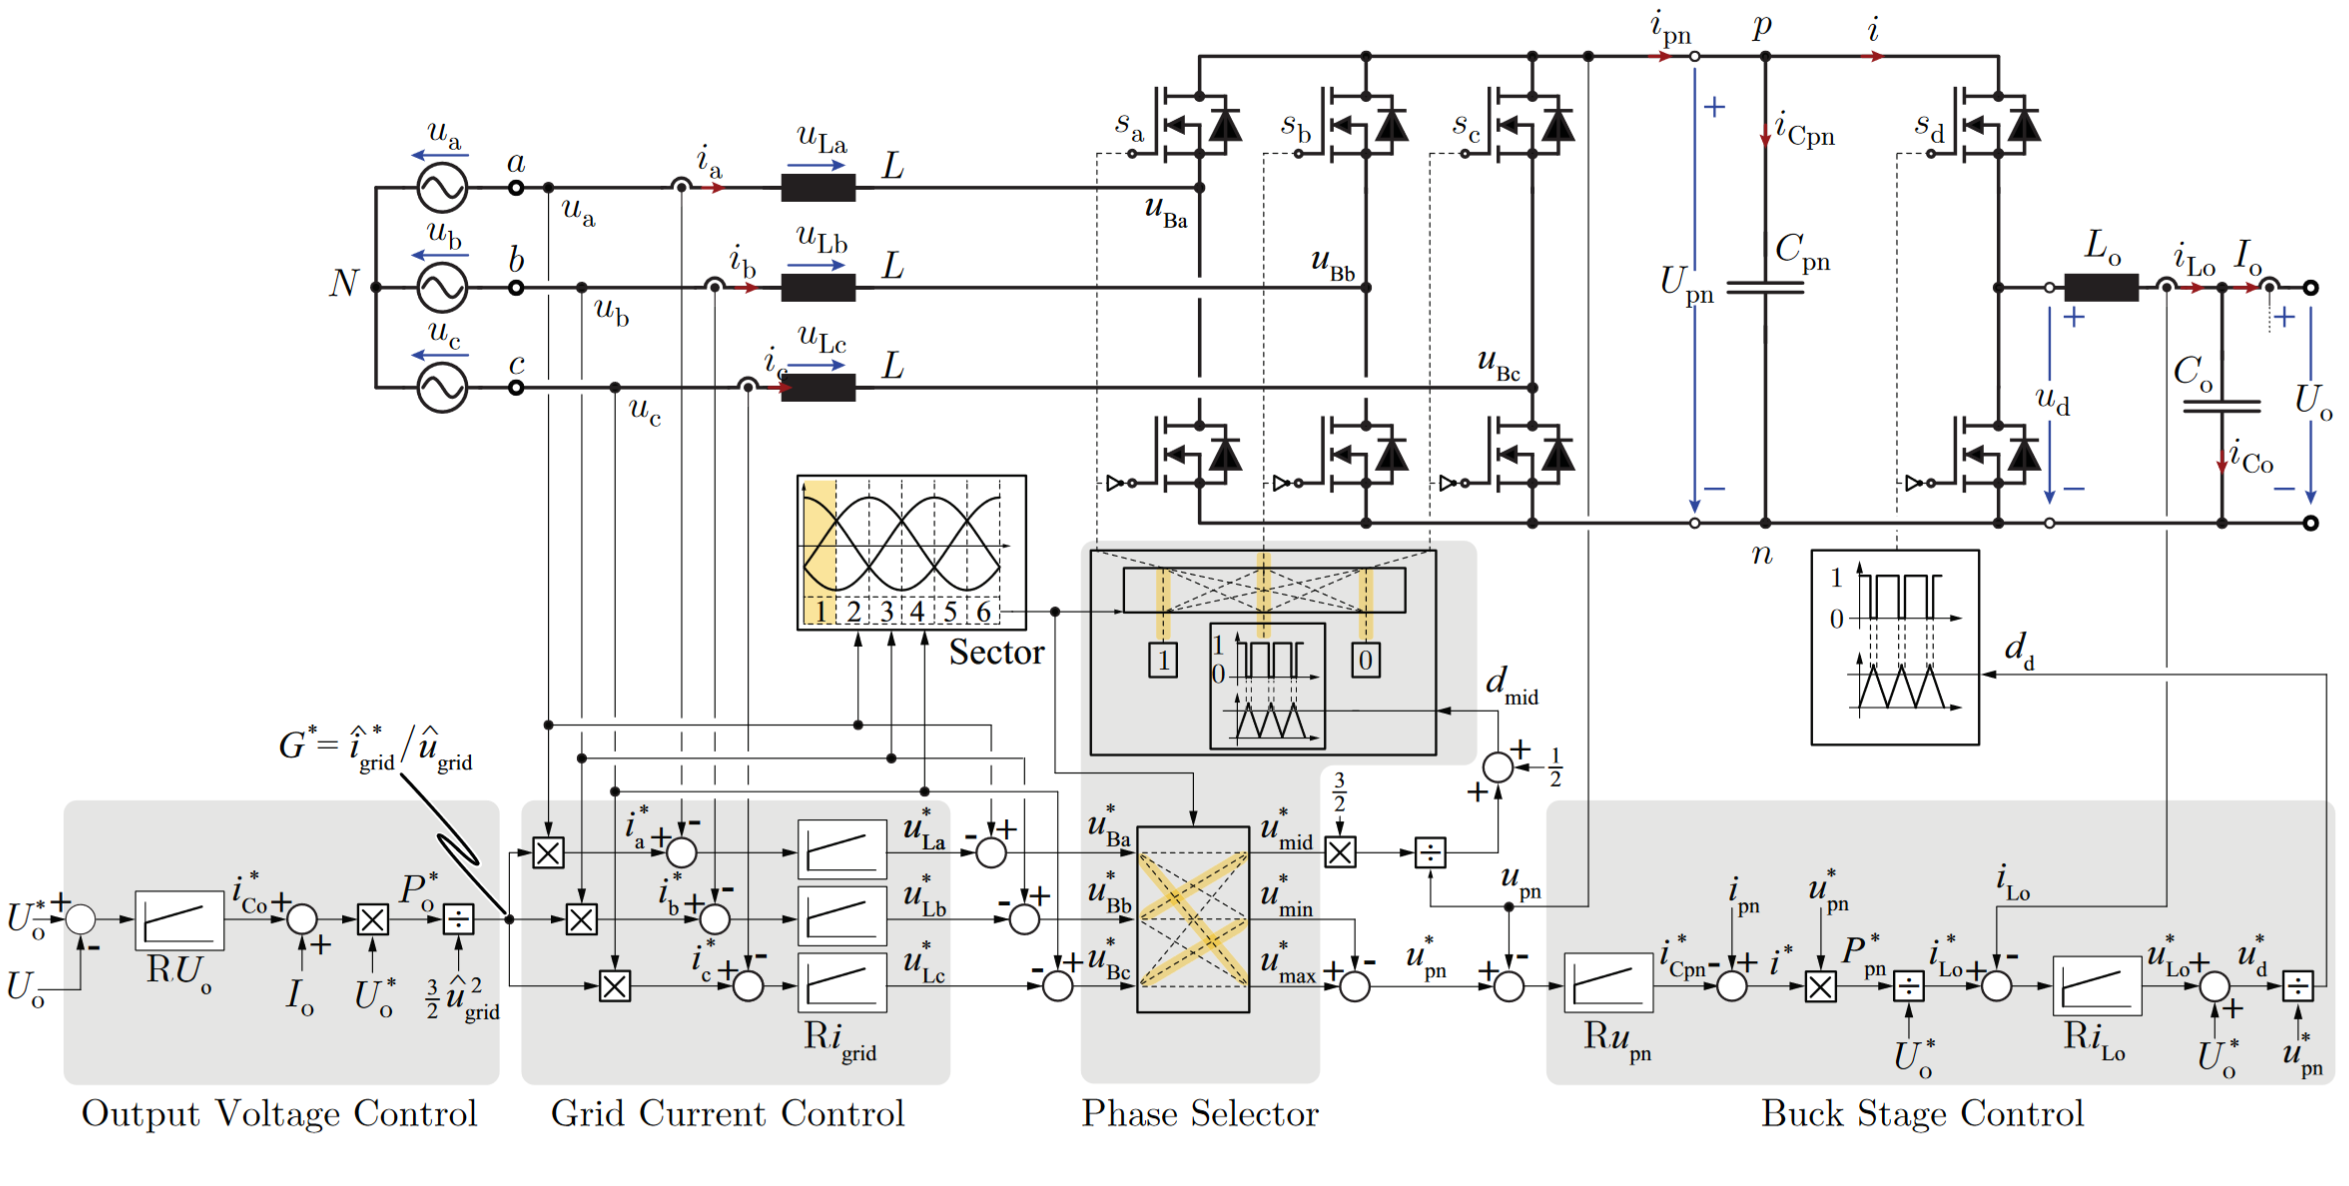
\includegraphics[width=1\linewidth]{content/Grafiken/B6-Control-orig}
			\caption{Regelung des \gls{B6PFC} \cite{13PWMPFC}}
			\label{fig:b6-control-orig}
			\end{figure}
		Die Ausgangsleistungsregelung in PLECS besteht aus einem PI-Regler (siehe Abbildung \ref{fig:plecsb6controlpout}), der die nominale Netzspannung mit der äquivalenten Netzimpedanz multipliziert und dann durch die aktuelle Netzspannung in die Soll-Phasenströme umwandelt. Um die Phasenverschiebung zu implementieren, wird der Sollstrom entsprechend des Phasenwinkels verzögert an die Regelung der B6-Ansteuerung weitergegeben.\\
				\begin{figure}
				\centering
				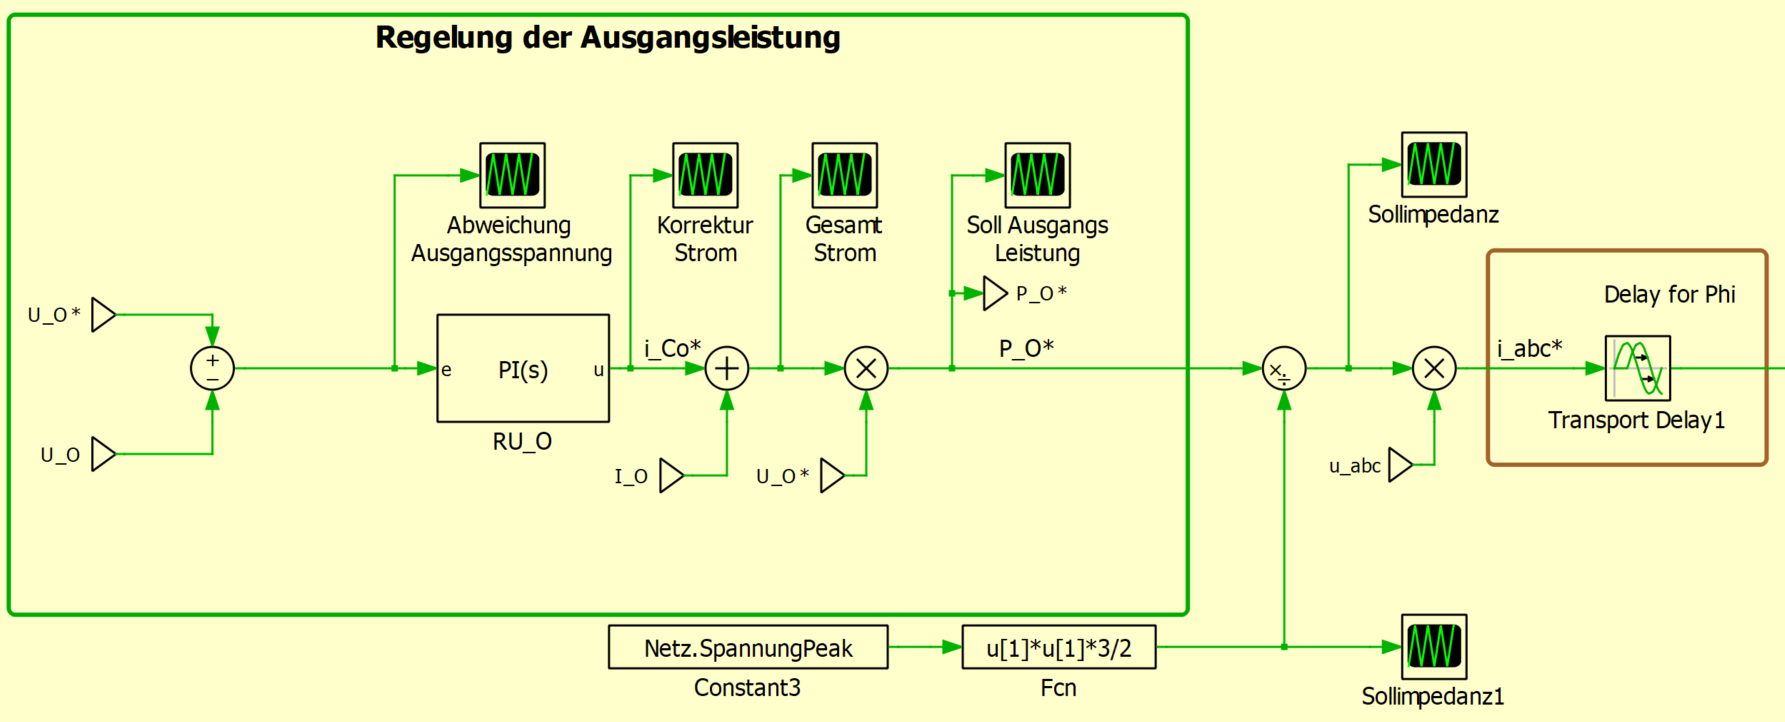
\includegraphics[width=0.9\linewidth]{content/Grafiken/PLECS_B6_ControlPout}
				\caption{PLECS Regelung der Ausgangsleistung als Sollgröße}
				\label{fig:plecsb6controlpout}
			\end{figure}
			Im nächsten Schritt wird die Regelung des Netzstroms durch einen weiteren PI-Regler implementiert. Die Erkennung der Phasenabschnitte wird mittels PLL und C-Skript umgesetzt. Siehe Abbildung \ref{fig:plecsb6controlrigrid}.  
				\begin{figure}
				\centering
				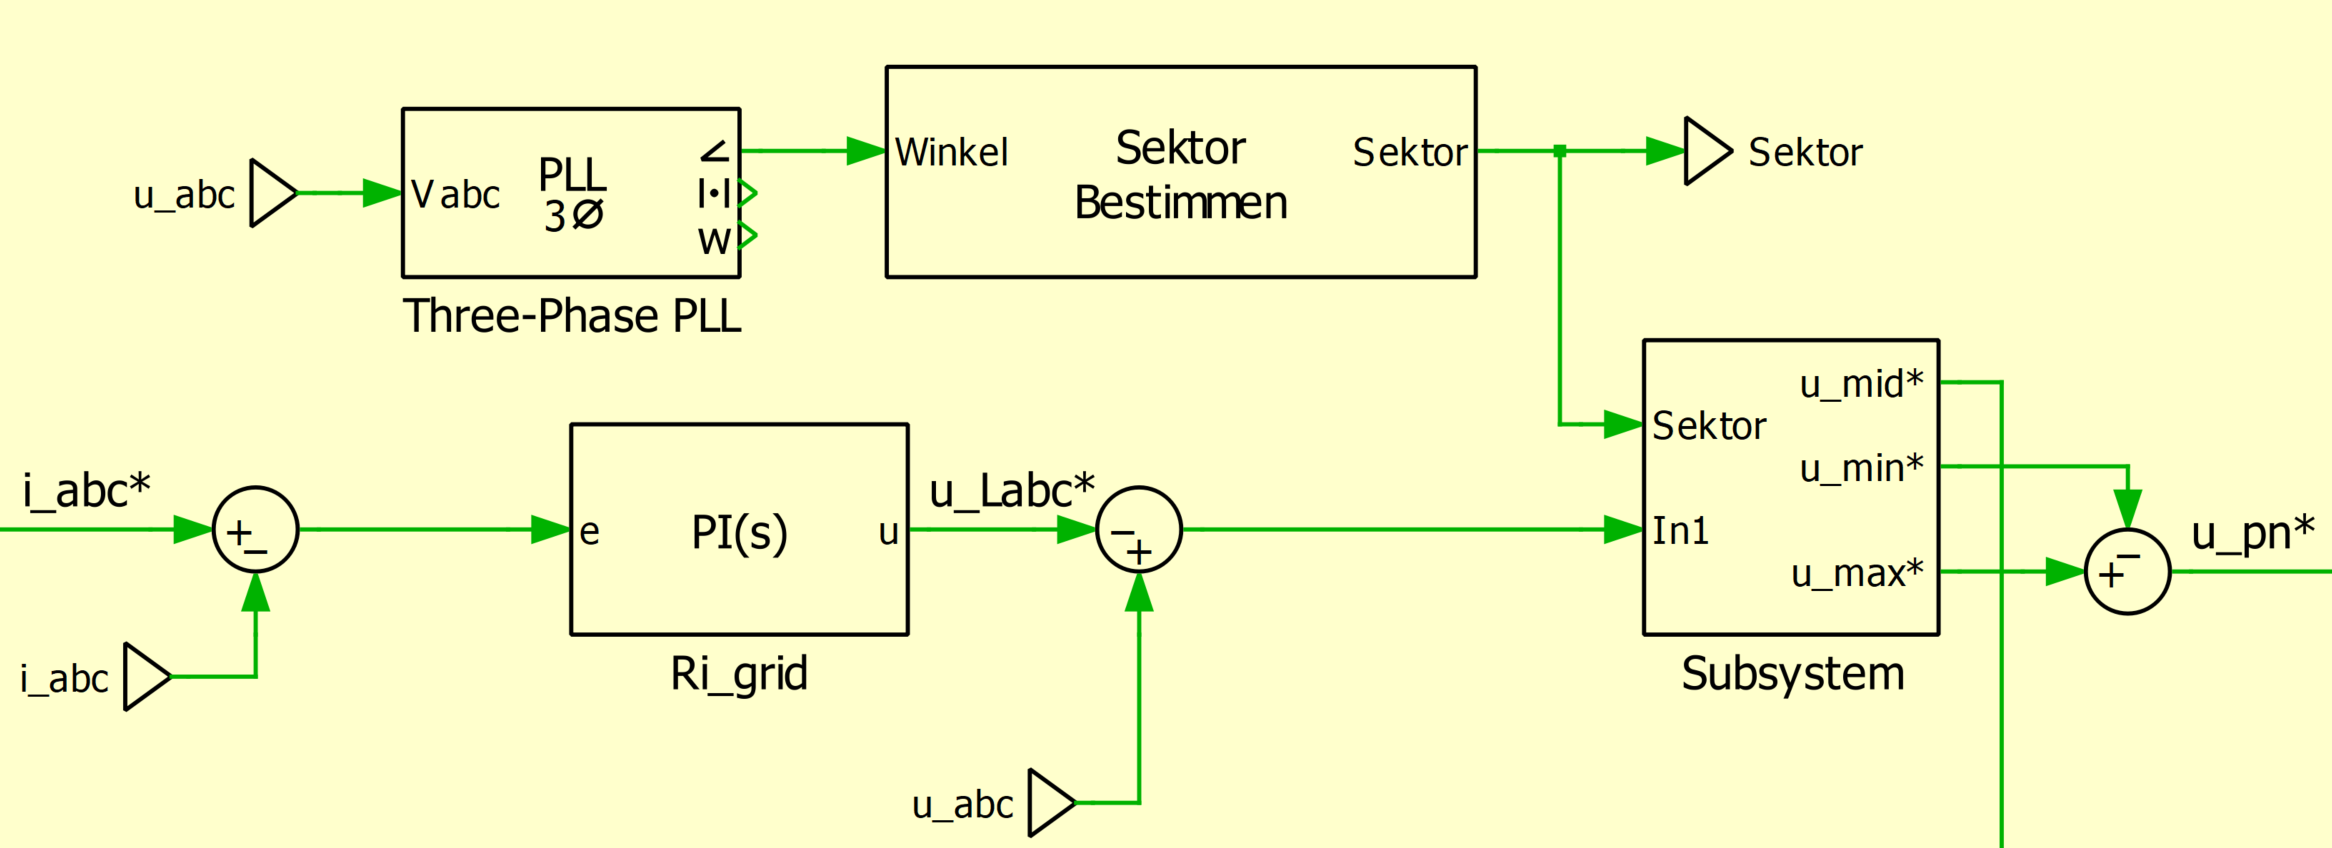
\includegraphics[width=0.9\linewidth]{content/Grafiken/PLECS_B6_ControlRiGrid}
				\caption{PLECS Regelung der Netzimpedanz und Phasenabschnittserkennung}
				\label{fig:plecsb6controlrigrid}
			\end{figure}
			Der Ausgang dieses Blocks dient einerseits mit der Sollgröße für die Zwischenkreisspannung $u\_pn*$ als Eingang für den Tiefsetzsteller und andererseits wird die Sollgröße der mittleren Spannung $u\_mid*$ als Eingang für die PWM-Erzeugung des \gls{B6PFC} Gleichrichters verwendet.\\
			Die Sollspannung der Mittenphase $U\_mid*$ dient als Eingangsgröße zur Erzeugung des PWM-Signals für die \gls{MOSFET}s. Dieses wird wiederum von einem PWM-Generator erzeugt und mit Hilfe eines C-Codes werden die Signale den entsprechenden Phasen im Sektor zugeordnet. Die Einschaltverzögerung dient der Totzeit-Implementierung, siehe Bild \ref{fig:plecsb6controlpwmmid}.\\
			\begin{figure}
				\centering
				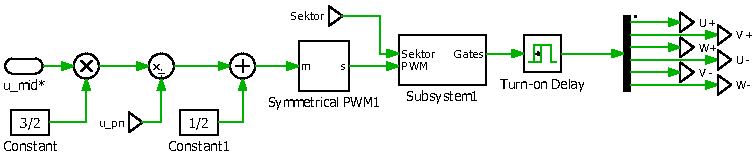
\includegraphics[width=0.9\linewidth]{content/Grafiken/PLECS_B6_ControlPWMmid}
				\caption{PLECS PWM Erzeugung des B6 Gleichrichters mit \gls{PFC}}
				\label{fig:plecsb6controlpwmmid}
			\end{figure}
			Die Ansteuerung des Tiefsetzstellers, siehe Abb. \ref{fig:b6buckcontrol}, wird hier wie in der Vorlage (in Abbildung \ref{fig:b6-control-orig} dargestellt) durch zwei PI-Regler realisiert. Im Gegensatz zur Variante des \gls{IAF} wird hier die Zwischenkreisspannung \gls{Upn} berücksichtigt. Als zusätzlicher Schritt wird das PWM-Signal erzeugt und die Totzeit der Halbleiter durch Verzögerungsfunktionen umgesetzt.  
\begin{figure}
	\centering
	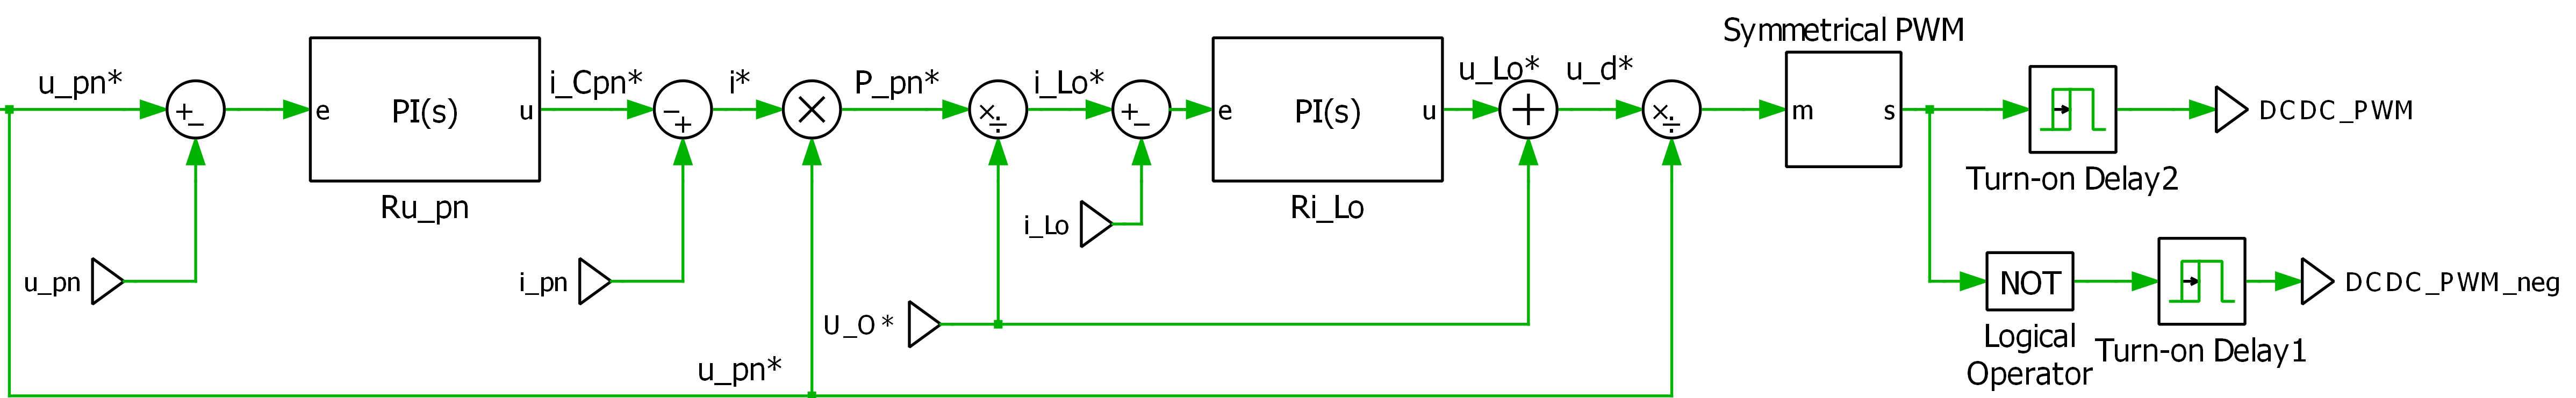
\includegraphics[width=1\linewidth]{content/Grafiken/B6_Buck_Control}
	\caption{Regelung des Tiefsetzstellers beim \gls{B6PFC}}
	\label{fig:b6buckcontrol}
\end{figure}		
\subsection{Ergebnisse}
			Es zeigt sich, dass der \gls{B6PFC} deutliche Nachteile bei den Induktivitäten und damit bei den Hardwarekosten hat. Die erforderliche dreiphasige Drossel führt dazu, dass der IAF in dieser Kategorie um mehr als 50\% besser abschneidet.
			Anders sieht es in den anderen Kategorien aus, wo weniger Kondensatoren benötigt werden. Die erforderliche B6-Schaltung enthält mehr \gls{MOSFET}, dafür aber keine Dioden. Bei der Verlustleistung zeigt sich der klare Vorteil der Topologie bei der Bereitstellung von \gls{SDL}, da sie fast keinen Einfluss auf die Verluste in den Halbleitern hat. Dies lässt sich anhand des Temperaturverhaltens in Abb. \ref{fig:b6temp030grad} bestätigen, durch die Reduzierung der Ausgangsleistung ist die Temperatur im \gls{MOSFET} FET7 des Tiefsetzsteller etwas niedriger, rosa dargestellt. Bei den Halbleitern der B6-Brücke ist praktisch kein Unterschied zu erkennen. Die Eingangsströme sind lediglich durch die Schaltimpulse leicht verrauscht und der Sinusverlauf folgt der Eingangsspannung wie gewünscht, siehe Abbildung \ref{fig:b6acdc0grad}.  Der Stromverlauf weist eine THD von nur etwa 5,8 \% auf.
			\begin{figure}
				\centering
				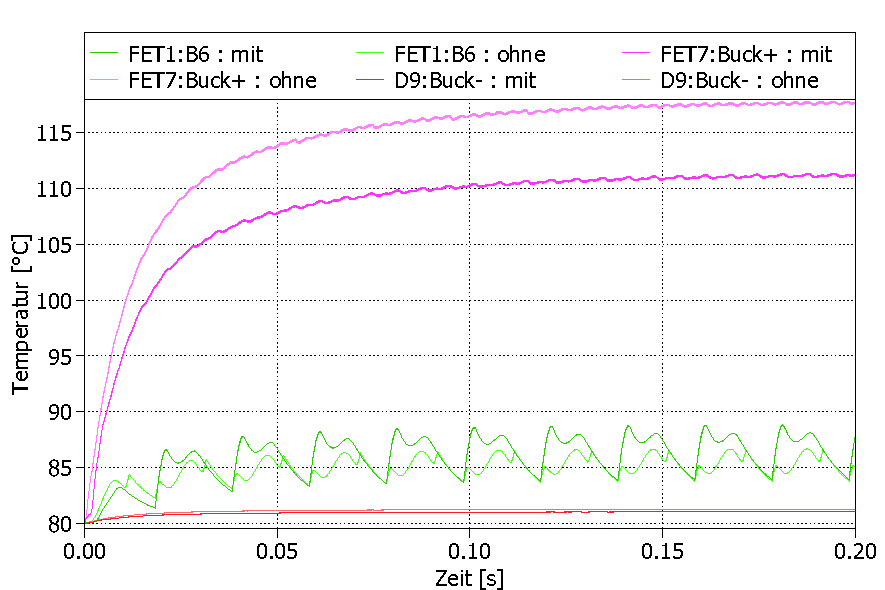
\includegraphics[width=1\linewidth]{content/Grafiken/B6_Temp_0&30Grad}
				\caption{Temperaturverhalten der Halbleiter des B6 mit und ohne Phasenverschiebung}
				\label{fig:b6temp030grad}
			\end{figure}
			\begin{figure}[H]
				\centering
				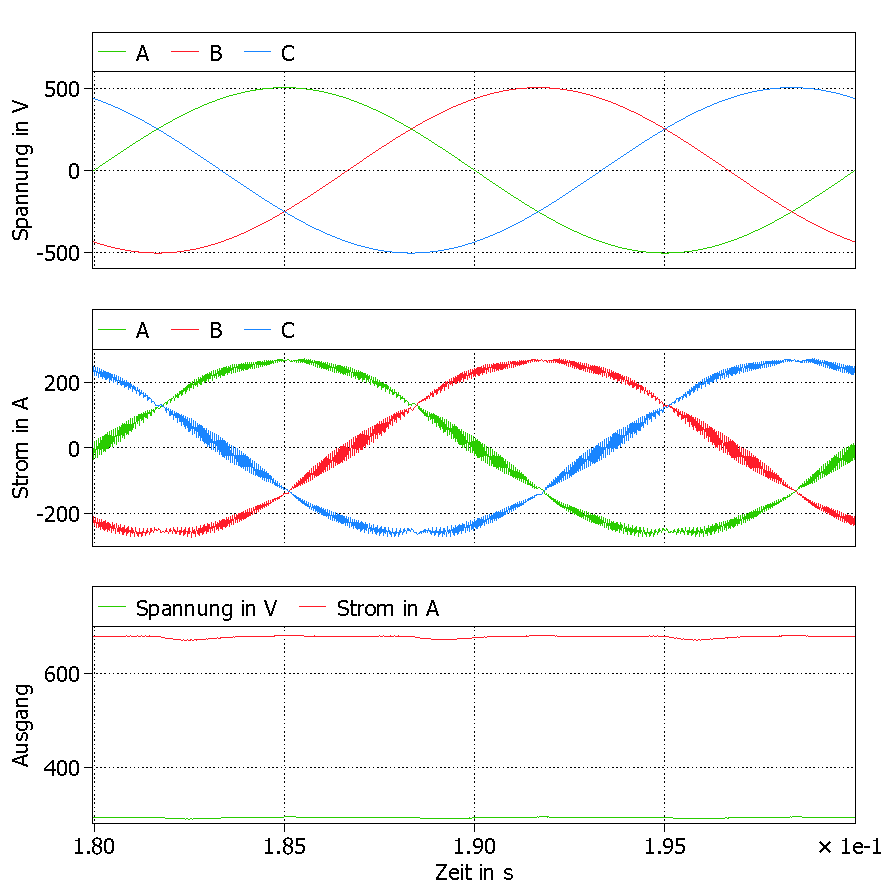
\includegraphics[width=1\linewidth]{content/Grafiken/B6_AC+DC_0Grad}
				\caption{Eingangs- und Ausgangsgrößen ohne Phasenverschiebung}
				\label{fig:b6acdc0grad}
			\end{figure}
			\pagebreak
			Mit einer Phasenverschiebung von 30 Grad sieht das Verhalten ähnlich aus, siehe Abbildung \ref{fig:b6acdc30grad}.  Der Stromverlauf weist eine etwas höhere THD von 7,1 \% auf, die jedoch durch geeignete Filter ausgeglichen werden kann.
			\begin{figure}
				\centering
				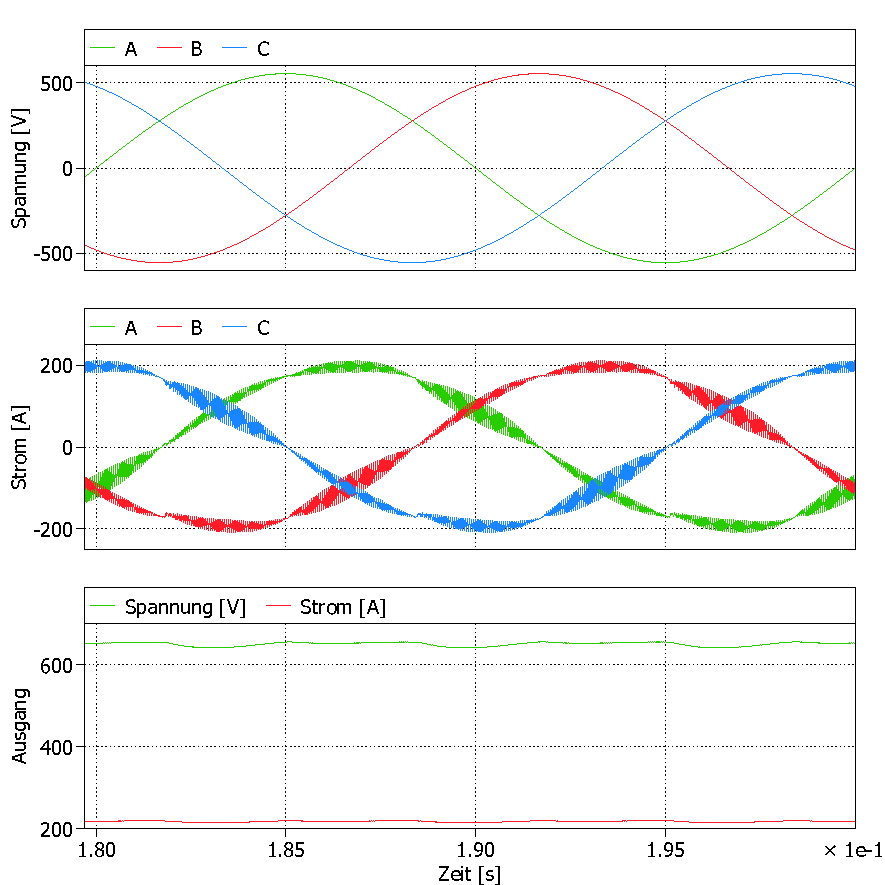
\includegraphics[width=1\linewidth]{content/Grafiken/B6_AC+DC_30Grad}
				\caption{Eingangs- und Ausgangsgrößen mit Phasenverschiebung}
				\label{fig:b6acdc30grad}
			\end{figure}
\section{Bewertung}
Die Ergebnisse der Gesamtbewertung sind in Tabelle \ref{tab:Auswertung} aufgeführt. Diese Tabelle enthält Informationen über die Hardware, insbesondere die Induktivitäten, sowie über die Kapazitäten, Halbleiter und Treiber. Zusätzlich werden die Ergebnisse der Simulation anhand der Verlustleistung der Halbleiter bewertet.  Zur Durchführung eines Vergleichs der Kategorien und einer Gesamtbewertung werden die Einzelkategorien zwischen null und eins normiert und mit einem Gewichtungsfaktor summiert. Die Kapazitäten haben nur einen vergleichsweise geringen Einfluss auf die Gesamtsystemkosten und werden daher nur mit fünf Prozent bewertet. Da die Drosseln einen größeren Einfluss haben, werden sie mit 50 Prozent gewichtet. Der Einfluss der Kondensatoren wird mit 5 Prozent berücksichtigt. Die restlichen 45 Prozent entfallen auf die Halbleiter in Form der Chipfläche (über den RDSON), die Anzahl der Treiber und die Verlustleistung. Die jeweiligen Punkte sind proportional zu erwartenden Systemkosten und Volumen. Daher stellt eine niedrigere Punktzahl eine bessere Bewertung dar. \\
\begin{table}
	\centering
	\caption{Auflistung der Simulationsergebnisse und Bewertung}
	\begin{tabular}{c|c|c|c|c}
		& Topologie & B6-Buck & \gls{IAF} & Gewichtung: \\
		\hline
		Induktivitäten& L1 Netzinduktivität \si{\micro \henry}& 136 & 1 &  \\
		\hline
		& Gespeicherte Energie J& 17,6 & 0,1 & \\
		\hline
		& L2 DC Induktivität \si{\micro \henry}& 136 & 136 &  \\
		\hline
		& Gespeicherte Energie J& 7,8 & 7,8 &  \\
		\hline
		& L3 IVS Induktivität \si{\micro \henry}& - & 302,2 &  \\
		\hline
		& Gespeicherte Energie J & - & 8,82 & \\
		\hline
		& \textbf{Induktivität normiert:} & \textbf{1}   & \textbf{0,66} & 50\% \\
		\hline
		Kapazitäten & C1 Netzkapazität \si{\micro \farad}& - & 50 &  \\
		\hline
		& C2 DC Ausgang mF& 1 & 1 &  \\
		\hline
		& C3 DC Zwischenkreis \si{\micro \farad}& 25 & 50 &  \\
		\hline
		& \textbf{Kapazität normiert:} & \textbf{0,26} &  \textbf{1} & 5\% \\
		\hline
		Halbleiter & SiC 4 \si{\milli \ohm} & 0 & 2 &  \\
		\hline
		& SiC 2 \si{\milli \ohm} & 10 & 4 &  \\
		\hline
		& SiC 5 \si{\milli \ohm} & 0 & 6 &  \\
		\hline
		& \textbf{MOSFET normiert:} & \textbf{1} &  \textbf{0,64} & 15\% \\
		\hline
		& Dioden & 0 & 6 &  \\
		\hline
		& \textbf{Dioden normiert} & \textbf{0} & \textbf{1} & 5\% \\
		\hline
		Treiber & Treiberanzahl & 8 & 7 &  \\
		\hline
		& \textbf{Treiber normiert:} & \textbf{1} & \textbf{0,88} & 5\% \\
		\hline
		Verluste in W & Schaltverluste 30 Grad & 567 & 503 &  \\
		\hline
		& Leitverluste 30 Grad & 254 & 1311 &  \\
		\hline
		& 30 Grad Gewichtung: & 75\% & 75\% &  \\
		\hline
		& Schaltverluste 0 Grad & 554 & 511 &  \\
		\hline
		& Leitverluste 0 Grad & 326 & 748 &  \\
		\hline
		& 0 Grad Gewichtung: & 25\% & 25\% &  \\
		\hline
		& \textbf{Verluste normiert:} &\textbf{0,5} & \textbf{1} & 20\% \\
		\hline
		\textbf{Gesamt} &  & \textbf{0,77} & \textbf{0,74} & \\
	\end{tabular}
	\label{tab:Auswertung}
\end{table}